\documentclass{article}

% \includegraphics
\usepackage{ifluatex}
\ifluatex
  \usepackage{pdftexcmds}
  \makeatletter
  \let\pdfstrcmp\pdf@strcmp
  \let\pdffilemoddate\pdf@filemoddate
  \makeatother
\fi
\usepackage{svg}
\usepackage{hyperref}
\usepackage{amsmath}
\usepackage{tikz}
\usepackage{tkz-graph}
\usepackage{pgf}
\usetikzlibrary{arrows,automata}

% For subfloat
\usepackage{subfig}


% For shell-escape
\usepackage[miktex]{gnuplottex}

\usepackage{scalerel}
\usepackage{stackengine,wasysym}


\usepackage{todonotes}

\title{The error when inferring phylogenies with incipient species by a Birth-Death model}
% \subtitle{Should protracted speciation be incorporated in phylogenetic tree construction methods?}

\author{Richel Bilderbeek}

% The functions used

% My first function, kept for nostalic reasons
\newcommand{\sayhello}{hello and howdy!}

% Making a note
\newcommand\note[1]{\textcolor{green}{\todo{#1}}}

% From https://tex.stackexchange.com/a/98034
\newcommand*\mean[1]{\overline{#1}}

% From https://tex.stackexchange.com/a/101138
% \newcommand\reallywidetilde[1]{\ThisStyle{%
%   \setbox0=\hbox{$\SavedStyle#1$}%
%   \stackengine{-.1\LMpt}{$\SavedStyle#1$}{%
%     \stretchto{\scaleto{\SavedStyle\mkern.2mu\AC}{.5150\wd0}}{.6\ht0}%
%   }{O}{c}{F}{T}{S}%
% }}

% Adapted from 'mean', use 'reallywidetilde'
% \newcommand*\median[1]{\reallywidetilde{#1}}

\newcommand*\median[1]{\widetilde{#1}}

%%%%%%%%%%%%%%%%%%%%%%%%%%%%%%%%%%%%%%%%%%%%%%%%%%%%%%%%%%%%%%%%%%%%%%%%%%%%%%%%
% Create the TikZ picture for fig:experiment
%%%%%%%%%%%%%%%%%%%%%%%%%%%%%%%%%%%%%%%%%%%%%%%%%%%%%%%%%%%%%%%%%%%%%%%%%%%%%%%%
\newcommand{\CreateTikzFigureExperiment} {

  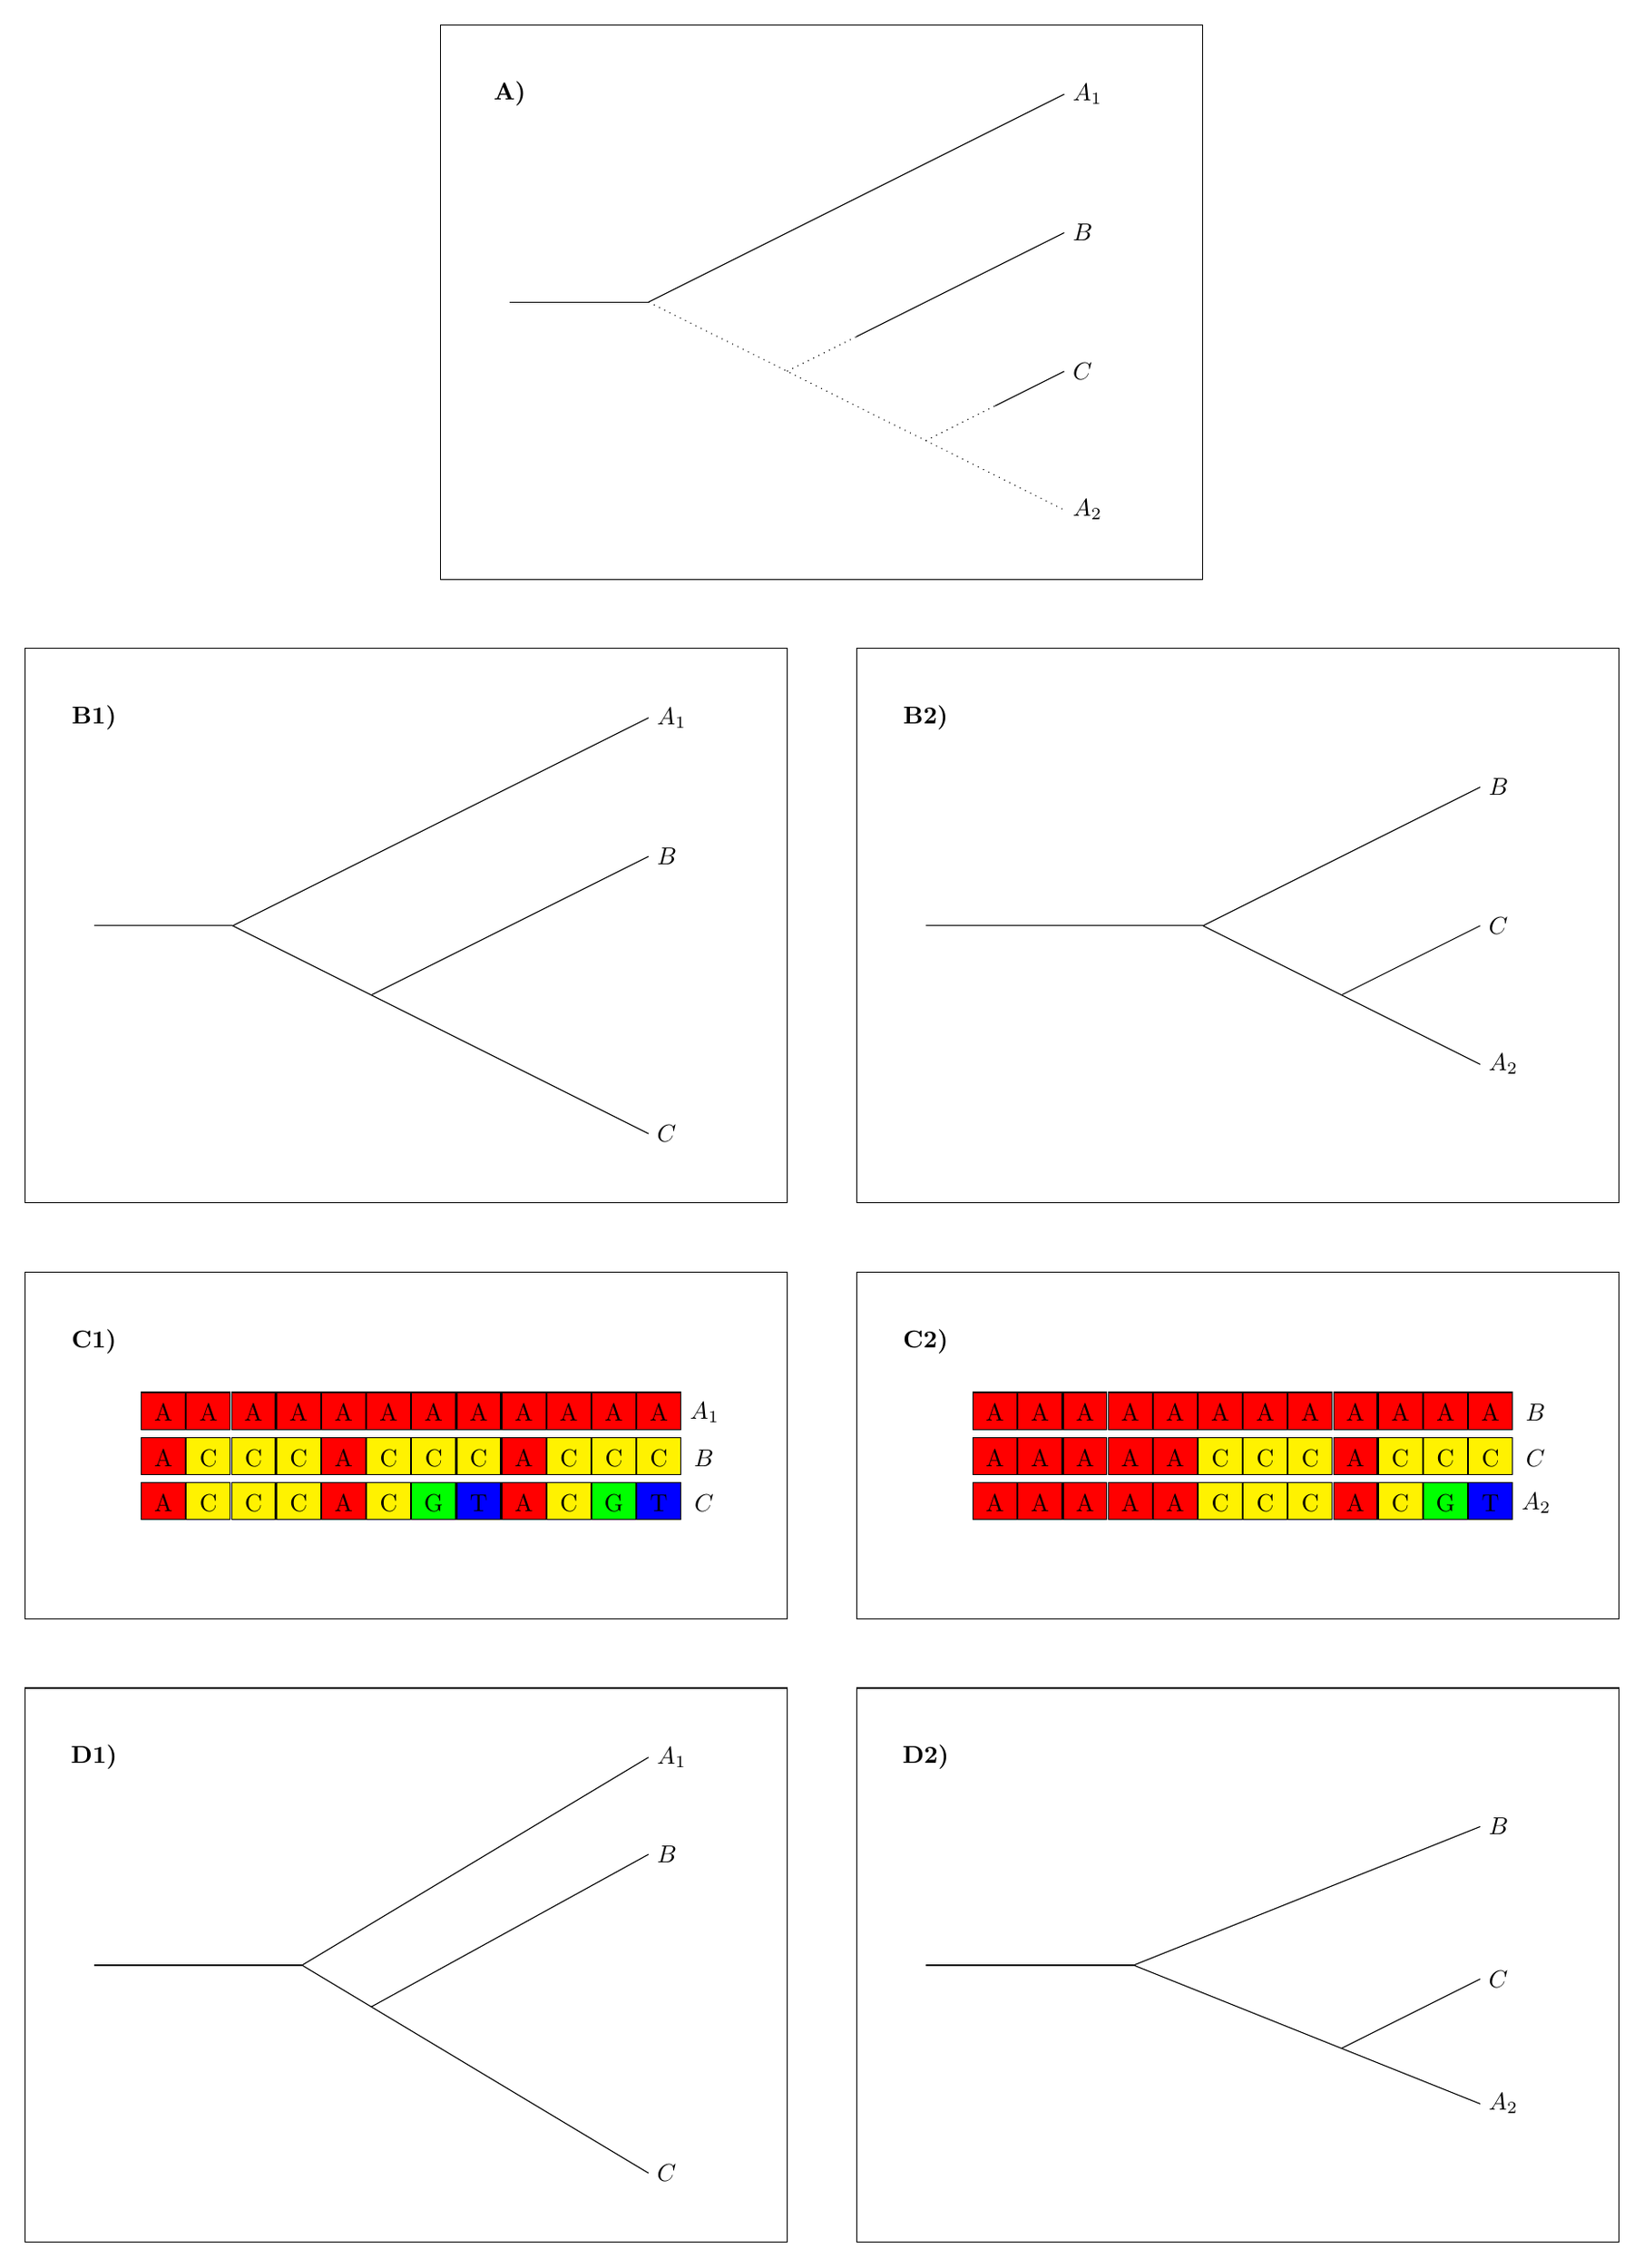
\begin{tikzpicture} 

    % Incipient species tree
    \begin{scope}[shift={(0,0)}] 

      \node[font = \bf] at (0, 0) {A)};
      \draw (-1,1) rectangle (10,-7);

      % Drawing of the phylogeny
      \begin{scope}[shift={(0,-3)}] 
        \draw (0, 0) -- (2,  0); % stem 
        \draw (2, 0) -- (8,  3) node[anchor=west] {$A_1$};
        \draw[dotted] (4,  -1) -- (5, -0.5); \draw (5, -0.5) -- (8, 1) node[anchor=west] {$B$};
        \draw[dotted] (6,  -2) -- (7, -1.5); \draw (7, -1.5) -- (8, -1) node[anchor=west] {$C$};
        \draw[dotted] (2,0) -- (8, -3) node[anchor=west] {$A_2$};
      \end{scope} % Drawing of the phylogeny

    \end{scope}


    % Species tree, oldest
    \begin{scope}[shift={(-6,-9)}] 

      \node[font = \bf] at (0.0, 0  ) {B1)};
      \draw (-1,1) rectangle (10,-7);

      % Drawing of the species tree, oldest
      \begin{scope}[shift={(0,-3)}] 
        \draw (0, 0) -- (2,  0); % stem 
        \draw (2, 0) -- (8,  3) node[anchor=west] {$A_1$};
        \draw (4,  -1) -- (8, 1) node[anchor=west] {$B$};
        \draw (2,0) -- (8, -3) node[anchor=west] {$C$};
      \end{scope} % Drawing of the species tree, oldest

    \end{scope}


    % Species tree, youngest
    \begin{scope}[shift={( 6,-9)}] 

      \node[font = \bf] at (0, 0) {B2)};
      \draw (-1,1) rectangle (10,-7);

      % Drawing of the species tree, youngest
      \begin{scope}[shift={(0,-3)}] 
        \draw (0, 0) -- (4,  0); % stem 
        \draw (4, 0) -- (8,  2) node[anchor=west] {$B$};
        \draw (6,-1) -- (8,  0) node[anchor=west] {$C$};
        \draw (4, 0) -- (8, -2) node[anchor=west] {$A_2$};
      \end{scope} % Drawing of the species tree, youngest

    \end{scope}

    % Alignment, oldest
    \begin{scope}[shift={(-6,-18)}] 

      \node[font = \bf] at (0.0, 0  ) {C1)};
      \draw (-1,1) rectangle (10,-4);

      % Drawing of the alignment
      \begin{scope}[shift={(1,-1)}, text width = 4mm, text height = 3mm, align = center, scale = 1.3] 

        \node[draw, fill = red   ] at (0.0, 0  ) {A};
        \node[draw, fill = red   ] at (0.5, 0  ) {A};
        \node[draw, fill = red   ] at (1.0, 0  ) {A};
        \node[draw, fill = red   ] at (1.5, 0  ) {A};
        \node[draw, fill = red   ] at (2.0, 0  ) {A};
        \node[draw, fill = red   ] at (2.5, 0  ) {A};
        \node[draw, fill = red   ] at (3.0, 0  ) {A};
        \node[draw, fill = red   ] at (3.5, 0  ) {A};
        \node[draw, fill = red   ] at (4.0, 0  ) {A};
        \node[draw, fill = red   ] at (4.5, 0  ) {A};
        \node[draw, fill = red   ] at (5.0, 0  ) {A};
        \node[draw, fill = red   ] at (5.5, 0  ) {A};
        \node[                   ] at (6.0, 0  ) {$A_1$};

        \node[draw, fill = red   ] at (0.0, -0.5) {A};
        \node[draw, fill = yellow] at (0.5, -0.5) {C};
        \node[draw, fill = yellow] at (1.0, -0.5) {C};
        \node[draw, fill = yellow] at (1.5, -0.5) {C};
        \node[draw, fill = red   ] at (2.0, -0.5) {A};
        \node[draw, fill = yellow] at (2.5, -0.5) {C};
        \node[draw, fill = yellow] at (3.0, -0.5) {C};
        \node[draw, fill = yellow] at (3.5, -0.5) {C};
        \node[draw, fill = red   ] at (4.0, -0.5) {A};
        \node[draw, fill = yellow] at (4.5, -0.5) {C};
        \node[draw, fill = yellow] at (5.0, -0.5) {C};
        \node[draw, fill = yellow] at (5.5, -0.5) {C};
        \node[                   ] at (6.0, -0.5) {$B$};

        \node[draw, fill = red] at (0.0, -1.0) {A};
        \node[draw, fill = yellow] at (0.5, -1.0) {C};
        \node[draw, fill = yellow] at (1.0, -1.0) {C};
        \node[draw, fill = yellow] at (1.5, -1.0) {C};
        \node[draw, fill = red   ] at (2.0, -1.0) {A};
        \node[draw, fill = yellow] at (2.5, -1.0) {C};
        \node[draw, fill = green ] at (3.0, -1.0) {G};
        \node[draw, fill = blue  ] at (3.5, -1.0) {T};
        \node[draw, fill = red   ] at (4.0, -1.0) {A};
        \node[draw, fill = yellow] at (4.5, -1.0) {C};
        \node[draw, fill = green ] at (5.0, -1.0) {G};
        \node[draw, fill = blue  ] at (5.5, -1.0) {T};
        \node[                   ] at (6.0, -1.0) {$C$};

      \end{scope} % Drawing of the alignment

    \end{scope}

    % Alignment, youngest
    \begin{scope}[shift={(6,-18)}] 

      \node[font = \bf] at (0.0, 0  ) {C2)};
      \draw (-1,1) rectangle (10,-4);

      % Drawing of the alignment
      \begin{scope}[shift={(1,-1)}, text width = 4mm, text height = 3mm, align = center, scale = 1.3] 

        \node[draw, fill = red   ] at (0.0, 0  ) {A};
        \node[draw, fill = red   ] at (0.5, 0  ) {A};
        \node[draw, fill = red   ] at (1.0, 0  ) {A};
        \node[draw, fill = red   ] at (1.5, 0  ) {A};
        \node[draw, fill = red   ] at (2.0, 0  ) {A};
        \node[draw, fill = red   ] at (2.5, 0  ) {A};
        \node[draw, fill = red   ] at (3.0, 0  ) {A};
        \node[draw, fill = red   ] at (3.5, 0  ) {A};
        \node[draw, fill = red   ] at (4.0, 0  ) {A};
        \node[draw, fill = red   ] at (4.5, 0  ) {A};
        \node[draw, fill = red   ] at (5.0, 0  ) {A};
        \node[draw, fill = red   ] at (5.5, 0  ) {A};
        \node[                   ] at (6.0, 0  ) {$B$};

        \node[draw, fill = red   ] at (0.0, -0.5) {A};
        \node[draw, fill = red   ] at (0.5, -0.5) {A};
        \node[draw, fill = red   ] at (1.0, -0.5) {A};
        \node[draw, fill = red   ] at (1.5, -0.5) {A};
        \node[draw, fill = red   ] at (2.0, -0.5) {A};
        \node[draw, fill = yellow] at (2.5, -0.5) {C};
        \node[draw, fill = yellow] at (3.0, -0.5) {C};
        \node[draw, fill = yellow] at (3.5, -0.5) {C};
        \node[draw, fill = red   ] at (4.0, -0.5) {A};
        \node[draw, fill = yellow] at (4.5, -0.5) {C};
        \node[draw, fill = yellow] at (5.0, -0.5) {C};
        \node[draw, fill = yellow] at (5.5, -0.5) {C};
        \node[                   ] at (6.0, -0.5) {$C$};

        \node[draw, fill = red   ] at (0.0, -1.0) {A};
        \node[draw, fill = red   ] at (0.5, -1.0) {A};
        \node[draw, fill = red   ] at (1.0, -1.0) {A};
        \node[draw, fill = red   ] at (1.5, -1.0) {A};
        \node[draw, fill = red   ] at (2.0, -1.0) {A};
        \node[draw, fill = yellow] at (2.5, -1.0) {C};
        \node[draw, fill = yellow] at (3.0, -1.0) {C};
        \node[draw, fill = yellow] at (3.5, -1.0) {C};
        \node[draw, fill = red   ] at (4.0, -1.0) {A};
        \node[draw, fill = yellow] at (4.5, -1.0) {C};
        \node[draw, fill = green ] at (5.0, -1.0) {G};
        \node[draw, fill = blue  ] at (5.5, -1.0) {T};
        \node[                   ] at (6.0, -1.0) {$A_2$};

      \end{scope} % Drawing of the alignment

    \end{scope}



    % Estimated species tree, oldest
    \begin{scope}[shift={(-6,-24)}] 

      \node[font = \bf] at (0, 0) {D1)};
      \draw (-1,1) rectangle (10,-7);

      \begin{scope}[shift={(0,-3)}] 
        \draw (0, 0) -- (3,  0);
        \draw (3, 0) -- (8, 3) node[anchor=west] {$A_1$};
        \draw (4,-0.6) -- (8, 1.6) node[anchor=west] {$B$};
        \draw (3, 0) -- (8,-3) node[anchor=west] {$C$};
      \end{scope}

    \end{scope}


    % Estimated species tree, youngest
    \begin{scope}[shift={(6,-24)}] 

      \node[font = \bf] at (0, 0) {D2)};
      \draw (-1,1) rectangle (10,-7);

      \begin{scope}[shift={(0,-3)}] 
        \draw (0, 0) -- (3,  0);
        \draw (3, 0) -- (8,  2) node[anchor=west] {$B$};
        \draw (6,-1.2) -- (8, -0.2) node[anchor=west] {$C$};
        \draw (3, 0) -- (8, -2) node[anchor=west] {$A_2$};
      \end{scope}

    \end{scope}

  \end{tikzpicture}
} % End of create_figure_experiment definition
%%%%%%%%%%%%%%%%%%%%%%%%%%%%%%%%%%%%%%%%%%%%%%%%%%%%%%%%%%%%%%%%%%%%%%%%%%%%%%%%




%%%%%%%%%%%%%%%%%%%%%%%%%%%%%%%%%%%%%%%%%%%%%%%%%%%%%%%%%%%%%%%%%%%%%%%%%%%%%%%%
% Create the TikZ picture of fig:sampling
%%%%%%%%%%%%%%%%%%%%%%%%%%%%%%%%%%%%%%%%%%%%%%%%%%%%%%%%%%%%%%%%%%%%%%%%%%%%%%%%
\newcommand{\CreateTikzFigureSampling} {

  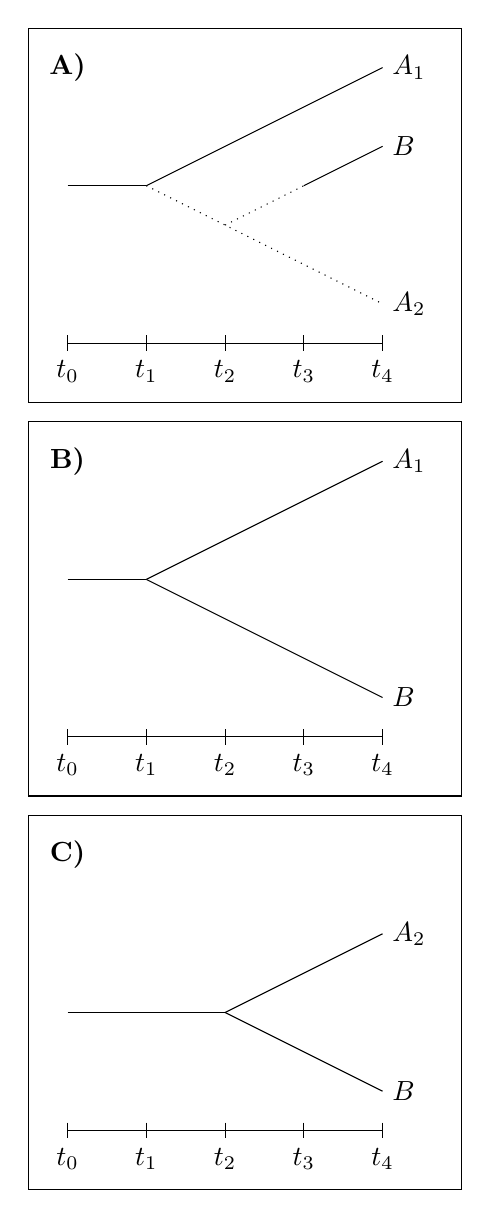
\begin{tikzpicture}[scale = 0.5] 

    \begin{scope}[shift={(0,0)}] 

      \node[font = \bf] at (0, 0) {A)};
      \draw (-1,1) rectangle (10,-8.5);

      % Drawing of the phylogeny
      \begin{scope}[shift={(0,-3)}] 
        \draw (0, 0) -- (2,  0);
        \draw (2, 0) -- (8,  3) node[anchor=west] {$A_1$};
        \draw[dotted] (2, 0) -- (8, -3) node[anchor=west] {$A_2$};
        \draw[dotted] (4, -1) -- (6, 0);
        \draw (6, 0) -- (8, 1) node[anchor=west] {$B$};
        % time scale
        \draw (0, -4) -- (8,  -4);
        \draw (0, -3.8) -- (0,  -4.2) node[anchor=north] {$t_0$};
        \draw (2, -3.8) -- (2,  -4.2) node[anchor=north] {$t_1$};
        \draw (4, -3.8) -- (4,  -4.2) node[anchor=north] {$t_2$};
        \draw (6, -3.8) -- (6,  -4.2) node[anchor=north] {$t_3$};
        \draw (8, -3.8) -- (8,  -4.2) node[anchor=north] {$t_4$};
      \end{scope} % Drawing of the phylogeny

    \end{scope}
    \begin{scope}[shift={(0, -10)}] 

      \node[font = \bf] at (0, 0) {B)};
      \draw (-1,1) rectangle (10,-8.5);

      % Drawing of the phylogeny
      \begin{scope}[shift={(0,-3)}] 
        \draw (0, 0) -- (2,  0);
        \draw (2, 0) -- (8,  3) node[anchor=west] {$A_1$};
        \draw (2, 0) -- (8, -3) node[anchor=west] {$B$};
        % time scale
        \draw (0, -4) -- (8,  -4);
        \draw (0, -3.8) -- (0,  -4.2) node[anchor=north] {$t_0$};
        \draw (2, -3.8) -- (2,  -4.2) node[anchor=north] {$t_1$};
        \draw (4, -3.8) -- (4,  -4.2) node[anchor=north] {$t_2$};
        \draw (6, -3.8) -- (6,  -4.2) node[anchor=north] {$t_3$};
        \draw (8, -3.8) -- (8,  -4.2) node[anchor=north] {$t_4$};
      \end{scope} % Drawing of the phylogeny

    \end{scope}
    \begin{scope}[shift={(0,-20)}] 

      \node[font = \bf] at (0, 0) {C)};
      \draw (-1,1) rectangle (10,-8.5);

      % Drawing of the phylogeny
      \begin{scope}[shift={(0,-3)}] 
        \draw (0, -1) -- (4, -1) ;
        \draw (4, -1) -- (8, -3) node[anchor=west] {$B$};
        \draw (4, -1) -- (8,  1) node[anchor=west] {$A_2$};
        % time scale
        \draw (0, -4) -- (8,  -4);
        \draw (0, -3.8) -- (0,  -4.2) node[anchor=north] {$t_0$};
        \draw (2, -3.8) -- (2,  -4.2) node[anchor=north] {$t_1$};
        \draw (4, -3.8) -- (4,  -4.2) node[anchor=north] {$t_2$};
        \draw (6, -3.8) -- (6,  -4.2) node[anchor=north] {$t_3$};
        \draw (8, -3.8) -- (8,  -4.2) node[anchor=north] {$t_4$};
      \end{scope} % Drawing of the phylogeny

    \end{scope}
  \end{tikzpicture}

} % End of create_figure_experiment definition
%%%%%%%%%%%%%%%%%%%%%%%%%%%%%%%%%%%%%%%%%%%%%%%%%%%%%%%%%%%%%%%%%%%%%%%%%%%%%%%%



\begin{document}

\maketitle

\begin{abstract}
  The construction of phylogenies helps us answer evolutionary biological
questions.
Our current phylogenetic tools ignore the fact that speciation takes time,
which has an effect unknown in phylogeny reconstruction.
Here, we simulate true incipient species trees and their corresponding
DNA alignments, from which we measure the reconstruction of the phylogeny
using a standard birth-death model.
We measure the errors that the Bayesian phylogenetic software tool BEAST2
gives when recovering simulated phylogenies, for different times-to-speciate,
under a range of additional parameter settings.
It has been found that branch lengths are consistently and strongly 
underestimated for biologically relevant parameters.
This research shows that protractedness is a complexity of nature that
cannot always be ignored and should be incorporated in our phylogenetic
tools.

\end{abstract}

\section{Introduction}

% Biology: speciation takes time

It takes time for new species-to-be to achieve the status of a new species.
First, it takes time for the new species-to-be has 
to acquire sufficient different mutations to 
establish reproductive isolation \cite{schluter2001ecology}. Second, 
it takes time for us to recognize reproductive isolation
and reclassify that one single species has become two 
(or more) species. As an example, \cite{fennessy2016multi} 
showed that Africa has four instead of only one
giraffe species, with a common ancestor estimated 
at around 2 million years ago.

% The use of speciation models

From DNA sequences obtained in the present, we can construct phylogenies
to infer the evolutionary relationship between species and the time 
from which ancestral species developed into separate.
  
As we only sample DNA of extant species, 
we can only infer a reconstructed tree, in which
the lineages that have gone extinct are absent.
Although most models assume extinctions (\cite{yule1925mathematical} being the
classic exception, as at its time computation was expensive), 
information on extinction times is lost due to our sampling.


The time when reproductive isolation started to take off, is
also lost in our sampling method, if the new species-to-be is not 
recognized yet as such. Without fossil date, one cannot observe the
possibly many times that reproductive isolation built up, but was lost again.

% First model: constant rate birth death model

Although we know that speciation takes time, we commonly ignore this when
constructing a phylogeny, by choosing a constant-rate birth-death model
as a speciation model. This can be justified, as for lineages 
that have speciated far back in the past, there is no error. 
Yet in the present, we do not recognize the future species-to-be
that are already genetically converging, resulting in an underestimation
of the number of species present today, which can only be 
concluded in retrospect.

The constant-rate birth-death model (as described in for example \cite{nee1994reconstructed}) 
is among the simplest speciation models, and assumes a constant speciation
 rate $\lambda$ and constant extinction rate $\mu$.

Additionally, it assumes speciation is instantaneous.
The constant-rate birth-death model is popular for its simplicity, yet
has also served as a starting point for more elaborate speciation models.

% Other non-protracted speciation models

Other speciation models may assume that speciation rate changes in 
time \cite{rabosky2008explosive}, is dependent on the amount of species 
present \cite{etienne2011diversity}, or is trait dependent \cite{fitzjohn2009estimating}.

In these examples, the original birth-death model has been extended by making 
speciation rate dependent on time, diversity or trait value respectively.
The assumption that all these extensions share is that speciation is instantaneous;
that after a new branching event, both two lineages are (or are recognized as being) different
species.

% Protracted speciation model

% Good and incipient states

The protracted speciation model \cite{etienne2012prolonging} allows for speciation taking time.

It adds an additional species state (see also figure \ref{fig:pbd_states}),
coined the 'incipient' stage, which a lineages has to complete before becoming
a 'good' species.

One view is to say that good species have achieved reproductive isolation,
where incipient species are in the process of achieving this \todo{Add reference}.

As genetic drift is unlikely to be a relevant speciation mechanism,
this is more likely to be ecological speciation [Sobel et al., 2009]. 
\todo{RSE: Ben je het daarmee eens? Zou drift niet een belangrijke ooraak van speciation op islands kunnen zijn bijvoorbeeld?}

Alternatively, an incipient species can be described as a good-species-to-be,
yet not recognized as such \todo{?[Purvis et al., 2009]?}.

%%%%%%%%%%%%%%%%%%%%%%%%%%%%%%%%%%%%%%%%%%%%%%%%%%%%%%%%%%%%%%%%%%%%%%%%%%%%%%%%
\begin{figure}
  \centering
  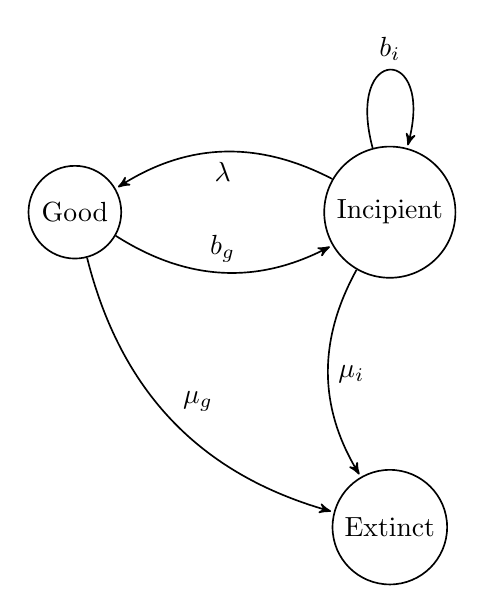
\begin{tikzpicture}[->,>=stealth',shorten >=1pt,auto,node distance=4cm, semithick]   
  \tikzstyle{every state}=[]
  \node[state] (A)              {Good};   
  \node[state] (B) [right of=A] {Incipient};   
  \node[state] (C) [below of=B] {Extinct};   
  \path (A) edge [bend right] node {$b_g$} (B)
        (A) edge [bend right] node {$\mu_g$} (C)
        (B) edge [loop above] node {$b_i$} (B)
        (B) edge [bend right] node {$\lambda$} (A)
        (B) edge [bend right] node {$\mu_i$} (C); 
  \end{tikzpicture}

  \caption{
    The states and transitions of a species in the PBD model.
    $b_i$: speciation-initiation rate of incipient species. 
    $b_g$: speciation-initiation rate of good species. 
    $\lambda$: speciation completion rate. 
    $\mu_i$: extinction rate of incipient species. 
    $\mu_g$: extinction rate of good species. 
    Figure after Etienne et al, 2014, Evolution
  }
  \label{fig:pbd_states}
\end{figure}
%%%%%%%%%%%%%%%%%%%%%%%%%%%%%%%%%%%%%%%%%%%%%%%%%%%%%%%%%%%%%%%%%%%%%%%%%%%%%%%%

% Biological mechanism of reproductive isolation

The protracted speciation model makes no assumption about the exact biological
mechanism by which reproductive isolation is 
acquired \cite{etienne2012prolonging, etienne2014estimating,rosindell2010protracted}.

A 'good' state can be viewed as a state in which there is convergent selection
for that lineage.

The 'incipient' state can be seen as a state in which there is the potential
for speciation.

A first example can be from the BDM \todo{Add reference} model, the state in which there
are all three genotypes, before the intermediate genotype is lost.
A second example can be in a sexual selection model [van Doorn and Weissing, 2002], 
where there is the onset for convergent selection.
In both cases, these intermediate states may fall back to the original
state of one species, or complete to produce a new species.

% Effects on topology

A feature of the protracted birth-death model, is that it may result in
paraphylies when the rates between good and incipient species differ \todo{Add reference}.
Paraphylies may be more than an experimental artifact and are claimed to
be an inherent feature of nature \cite{funk2003species}.

\todo{Add something like: this research solves this by sampling from paraphyletic trees (at the subspecies level) to create non-paraphyletic trees at the species level}

% Good and incipient rates

Where the classic birth death model assumes constant speciation and extinction
 rates, the protracted birth-death model allows these rates to be state
 dependent.

The only additional parameter is the rate at which incipient species become
(recognized as) good species.
When setting that parameter to infinity, incipient species become good
species instantaneous and the model falls back to a constant-rate (non-protracted) birth-death model \todo{Add reference}.

% Relationship to constant-rate birth-death model

\todo{?Wat bedoelde ik met deze onzin?}
Although both standard and protracted birth-death models use a parameter 
$\lambda$, the $\lambda$ in the standard birth death model denotes
a speciation rates (initiation and completion), where in the PBD model
$\lambda$ denotes only the speciation initiation rate. 
There is no relationship known between the parameters of the constant-rate
birth-death model and the protracted birth-death model \cite{etienne2014estimating} 
\todo{refesh memory, then update paragraph}.

% Good and incipient rates do not need to be constant

The assumption that speciation takes time is independent of the dynamics
of the speciation and extinction rates.
The protracted speciation model in this research assumes these rates are
constant, but these rates can easily be made to depend on time, diversity
or trait.

% Use of a speciation model in inferring a phylogeny

Speciation models are widely used to make inferences from genetic data.
There are multiple computer programs to create phylogenies and/or parameter
estimates from aligned DNA sequences.
BEAST2 is a widely used tool that allows for a Bayesian approach to 
phylogenetics \cite{bouckaert2014beast}.

BEAST2 supplies the user with multiple speciation models, that all assume
instantaneous speciation.
 
% This study

This simulation investigates the consequence of BEAST2 using instantaneous
speciation, by simulating a 'true' tree that is protracted, simulate DNA
alignments following that tree, and seeing how well BEAST2 can recover
the original phylogeny.
 
% Novelty

This study is the first to measure the error made when acknowledging that
speciation takes time, yet using one of the many tools that ignores this
fact.



Part of the parameter space will create 'true' trees that are not protracted.
This will result in a test of BEAST2 against itself, which is, to the best
of our knowledge, not been done, probably due to the extensive computations
that are needed \todo{RSE: Heb je dit uitgebreid getest? Misschien zou je Remco kunnen vragen}.

% Analysis

The 'true' and inferred trees are compared with the nLTT statistic, which
is a novel and efficient summary statistic, that has been proven to have
better performance than the gamma statistics in Approximate
Bayesian Computation \cite{janzen2015approximate} (yet on par with the likelihood).

The nLTT statistics is the summed absolute difference between two 
Lineages-Through-Time plot lines that are normalized to 
let both time and number of lineages
range from zero to one.
Additionally, this statistic allows to pinpoint the time span that contributed
most to its value.

% Expectations

It is expected that for higher protractedness (thus deviation from BEAST2
its assumptions), the error will increase.
Trees are expected to be inferred better, when there is more information
available to construct them, thus we expect less error when there are more
taxa and when the simulation DNA alignments are longer.
The error is expected to be biggest close to the present, as there will
be the most incipient species present.
 
It is unknown, however, under which biological settings this error is relevant.

% Preview results

This study shows that ... \todo{put result here}.


%%%%%%%%%%%%%%%%%%%%%%%%%%%%%%%%%%%%%%%%%%%%%%%%%%%%%%%%%%%%%%%%%%%%%%%%%%%%%%%%
\section{Methods}
%%%%%%%%%%%%%%%%%%%%%%%%%%%%%%%%%%%%%%%%%%%%%%%%%%%%%%%%%%%%%%%%%%%%%%%%%%%%%%%%

This research measures the error our current BD tools make, when
the real process has been protracted. Figure \ref{fig:experiment} shows
the following overview of the experiment graphically.
 An in silico data set is created for a wide
range of parameters from which incipient species trees are simulated (A in figure \ref{fig:experiment}). 
These phylogenies serve as 'the truth' or 'nature'. From that incipient species tree,
species trees are created, by picking one representive per species.
This is done twice, as either the youngest (B1) or oldest (B2) subspecies is chosen
to represent a species. Per species tree, $n_a$ alignments are simulated (C1 and C2).
Per alignment, $n_b$ posteriors are inferred, 
each consisting of $n_s$ phylogenies and parameter estimates (D1 and D2). Each
species tree is then compared with the species tree its alignment is based on (for
example, B1 and D1).

%%%%%%%%%%%%%%%%%%%%%%%%%%%%%%%%%%%%%%%%%%%%%%%%%%%%%%%%%%%%%%%%%%%%%%%%%%%%%%%%
\begin{figure}
  \centering 
  \resizebox {0.8\textwidth} {!} {
    \CreateTikzFigureExperiment{} 
  }
  \caption{
    Overview of the experiment: 
    A: per parameter set, there are $n_i$ incipient species trees created. 
    B1: constructing a species trees by using the youngest subspecies $A1$ to represent good species $A$.
    B2: constructing a species trees by using the oldest subspecies $A2$ to represent good species $A$.
    C1: constructing one of the $n_a$ alignments of B1. 
    C2: constructing one of the $n_a$ alignments of B2. 
    D1: reconstructing a species trees from alignment B1.
    D2: reconstructing a species trees from alignment B2.
    Comparisons are done between a species tree and its reconstructed species tree, 
    for example, between B1 and D1.
    All phylogenies are drawn at the same scale.
  }
  \label{fig:experiment}
\end{figure}
%%%%%%%%%%%%%%%%%%%%%%%%%%%%%%%%%%%%%%%%%%%%%%%%%%%%%%%%%%%%%%%%%%%%%%%%%%%%%%%%

%%%%%%%%%%%%%%%%%%%%%%%%%%%%%%%%%%%%%%%%%%%%%%%%%%%%%%%%%%%%%%%%%%%%%%%%%%%%%%%%
\subsection{Parameter space}
\label{subsec:parameter_space}
%%%%%%%%%%%%%%%%%%%%%%%%%%%%%%%%%%%%%%%%%%%%%%%%%%%%%%%%%%%%%%%%%%%%%%%%%%%%%%%%

%%%%%%%%%%%%%%%%%%%%%%%%%%%%%%%%%%%%%%%%%%%%%%%%%%%%%%%%%%%%%%%%%%%%%%%%%%%%%%%%
\begin{table}
  \centering 
  \begin{tabular}{l l}
    \hline
    Symbol & Description \\
    \hline
    \hline
    $b_g$ & Speciation initiation rate of a good species (probability per lineage, per million year) \\
    $b_i$ & Speciation initiation rate of an incipient species (probability per lineage, per million year) \\
    $\lambda$ & Speciation completion rate (probability per lineage, per million year) \\
    $\mu_g$ & Extinction rate of a good species (probability per lineage, per million year) \\
    $\mu_i$ & Extinction rate of an incipient species (probability per lineage, per million year) \\
    \hline
    $t_c$ & Crown age (million years) \\
    $r$ & Mutation rate (probability of mutation per nucleotide per million years) \\
    $l_a$ & DNA alignment length (base pairs) \\
    \hline
    $n_i$ & Number of incipient species trees per parameter set \\
    $n_a$ & Number of alignments per species tree \\
    $n_b$ & Number of BEAST2 runs per alignment \\
    \hline
    $n_s$ & Number of MCMC samples \\
    $i_s$ & MCMC sampling interval \\
    \hline
    $n_{ti}$ & Number of taxa in an incipient species tree \\
    $n_{t}$ & Number of taxa in a (good) species tree \\
    $t_{\mean{ds}}$ & Average duration of speciation \\
    $t_{sc}$ & Speciation completion time \\
    $\Delta_{nLTT}$ & nLTT statistic value \\
    $\mean{\Delta_{nLTT}}$ & Average nLTT statistic value of a posterior \\
    $\median{\Delta_{nLTT}}$ & Median nLTT statistic value of a posterior \\
    \hline
  \end{tabular}
  \caption{
    Parameter descriptions. The sections are (1) the biological parameters, (2) the
    biological tuning parameters, (3) parameters involved in replication, (4) MCMC
    tuning parameters, and (5) other symbols.
  }
  \label{table:parameter_descriptions}
\end{table}
%%%%%%%%%%%%%%%%%%%%%%%%%%%%%%%%%%%%%%%%%%%%%%%%%%%%%%%%%%%%%%%%%%%%%%%%%%%%%%%%

\todo{@RSE: would you prefer $t_{\mean{ds}}$ or $\mean{t_{ds}}$ for average duration of speciation?}

%%%%%%%%%%%%%%%%%%%%%%%%%%%%%%%%%%%%%%%%%%%%%%%%%%%%%%%%%%%%%%%%%%%%%%%%%%%%%%%%
\begin{table}
  \centering 
  \begin{tabular}{l l}
    \hline
    Parameter             & Values \\
    \hline
    \hline
    $b = b_g = b_i$       & 0.1, 0.5, 1.0 \\
    $\lambda$             & 0.1, 0.3, 1.0, $10^6$ \\
    $\mu = \mu_g = \mu_i$ & 0.0, 0.1, 0.2, 0.4 \\
    \hline
    $t_c$                 & 15 \\
    $r$                   & 0.01 \\
    $l_a$                 & $10^3$, $10^4$ \\
    \hline
    $n_i$                 & 20 \\
    $n_a$                 & 2 \\
    $n_b$                 & 2 \\
    \hline
    $n_s$                 & $10^3$ \\
    $i_s$                 & $10^3$ \\
    \hline
  \end{tabular}
  \caption{
    Parameter values. The sections are (1) the biological parameters, (2) the
    biological tuning parameters, (3) parameters involved in replication, 
    and (4) MCMC tuning parameters.
  }
  \label{table:parameter_values}
\end{table}
%%%%%%%%%%%%%%%%%%%%%%%%%%%%%%%%%%%%%%%%%%%%%%%%%%%%%%%%%%%%%%%%%%%%%%%%%%%%%%%%

% Biological parameters

This study primarily investigates combinations of the five biological 
parameters ($b_g$, $b_g$, $\lambda$, $\mu_g$ and $\mu_g$, 
see also figure \ref{fig:pbd_states} and table \ref{table:parameter_descriptions}), 
in a close to full factorial fashion, with two exceptions.
First, following \cite{etienne2014estimating}, birth and extinction rates were each 
set equal between good and incipient species ($b_g = b_i$, and $\mu_g = \mu_i$).
Second, only parameter combinations with speciation initiation rates greater
than extinction rates were used ($b_g > \mu_g$). The values 
used in the experiment (see table \ref{table:parameter_values}) 
were selected to have a reasonable expected number of incipient 
lineages, $E(n_{ti})$, where \todo{?too basic to have a reference to? I assume Kendall, 1948, \cite{kendall1948generalized}, but could not look it up here and now}: 

\begin{equation}
  E(n_{ti}) = e^{ (b - \mu) \cdot t_c }
\end{equation}

One value of speciation completion rate $\lambda$ is set (close to) infinity, as
then the protracted speciation model falls back to a constant-rate 
(non-protracted) birth-death model [?Etienne et al., 2012 or already Rosindell and Etienne 2011?].

% Biological tuning parameters

Secondarily, there are three biological tuning parameters. The crown age of
the incipient species tree, $t_c$, is set to 15 million years for all simulations, 
following \cite{etienne2014estimating}. The per-nucleotide mutation rate, $r$, and the
DNA aligment length, $l_a$, together must be tuned to result in informative
DNA alignments (see section \ref{subsec:simulating_alignments}). $r$ is identical in all
simulations. Increasing $l_a$ results in more informative alignments, and this
effect is measured by using two values of $l_a$ 
per biological parameter combination.

% Replication parameters

All processes involving stochasticity have replicates. 
For each set of parameters, $n_i$ incipient species trees are simulated. 
From each species tree, $n_a$ alignments are simulated. From each alignment, 
$n_b$ posteriors are generated.

% MCMC tuning parameters

The posteriors are generated using BEAST2, which uses a Monte-Carlo Markov-Chain (MCMC)
algorithm. This algorithm is tuned to result in a high effective sample size (ESS) by
two constants. The first constant is the MCMC sampling interval, which is $i_s$ states.
$i_s$ which must be high enough to avoid correlation between subsequently sampled posterior states.  
The second constant is the number of MCMC state samples, $n_s$, which equals the ESS iff \todo{@RSE: Can I use iff?}
$i_s$ is high enough to have no correlation between subsequently sampled posterior states.

%%%%%%%%%%%%%%%%%%%%%%%%%%%%%%%%%%%%%%%%%%%%%%%%%%%%%%%%%%%%%%%%%%%%%%%%%%%%%%%%
\subsection{Simulating incipient species trees}
\label{subsec:simulating_incipient_species_trees}
%%%%%%%%%%%%%%%%%%%%%%%%%%%%%%%%%%%%%%%%%%%%%%%%%%%%%%%%%%%%%%%%%%%%%%%%%%%%%%%%

From each parameter set, $n_i$ incipient species trees with a crown age
of $t_c$ and at least two extant taxa, 
are created in R \cite{R} using the PBD package \cite{PBD}.
The values of the biological parameters encourage that the number of tips in
each phylogeny is kept within computational limits. However, due to
the stochastic nature of the Doob-Gillespie algorithm used in the creation
of these phylogenies, phylogenies can, by chance, become very big. 
There is no maximum number of taxa set, yet imposed instead by the R 
programming language itself, due to a limit on the amount of memory that can be 
allocated. The incipient species trees that could not be simulated are
counted and discarded from further analysis.  

%%%%%%%%%%%%%%%%%%%%%%%%%%%%%%%%%%%%%%%%%%%%%%%%%%%%%%%%%%%%%%%%%%%%%%%%%%%%%%%%
\subsection{Sampling species trees}
\label{subsec:sampling_species_trees}
%%%%%%%%%%%%%%%%%%%%%%%%%%%%%%%%%%%%%%%%%%%%%%%%%%%%%%%%%%%%%%%%%%%%%%%%%%%%%%%%

Per incipient species tree, two species trees are created. 
To create a species tree (a tree in which each species is represented once)
for an incipient species tree, one representative for each species is picked. 
If a species has initiated one or more incipient species, either the youngest
or the oldest representative is picked. See figure \ref{fig:sampling} for an example.

An alternative sampling method would be to pick 
random representatives of each species. This would decrease the variability
between the two species tree. Maximizing variability between the two
species trees allows for clearer measuments on the effect of sampling.   

%%%%%%%%%%%%%%%%%%%%%%%%%%%%%%%%%%%%%%%%%%%%%%%%%%%%%%%%%%%%%%%%%%%%%%%%%%%%%%%%
\begin{figure}
  \centering 
  \CreateTikzFigureSampling{}
  \caption{
    Sampling an incipient species tree. 
    A) At stem age $t_0$, $A1$ is present.
    At crown age $t_1$, its derived incipient species $A2$ is born. 
    At $t_2$, $A2$ itself speciates into a new (unnamed) species, 
    that becomes good species $B$ at $t_3$. At present time, $t_4$, there
    exist two possible representatives of species $A$. 
    B) Using the oldest representative, $A1$, to represent species $A$, the crown
    age of the resulting species tree lies at $t_1$. 
    C) Using the youngest representative, $A2$, to represent species $A$, the crown
    age of the resulting species tree lies at $t_2$. 
  }
  \label{fig:sampling}
\end{figure}
%%%%%%%%%%%%%%%%%%%%%%%%%%%%%%%%%%%%%%%%%%%%%%%%%%%%%%%%%%%%%%%%%%%%%%%%%%%%%%%%

%%%%%%%%%%%%%%%%%%%%%%%%%%%%%%%%%%%%%%%%%%%%%%%%%%%%%%%%%%%%%%%%%%%%%%%%%%%%%%%%
\subsection{Simulating alignments}
\label{subsec:simulating_alignments}
%%%%%%%%%%%%%%%%%%%%%%%%%%%%%%%%%%%%%%%%%%%%%%%%%%%%%%%%%%%%%%%%%%%%%%%%%%%%%%%%

From each species tree, $n_a$ DNA alignments were simulated that match the
phylogeny's structure, using the phangorn R package \cite{phangorn}. 
Each alignment contains one DNA sequence per species 
of $l_a$ nucleotides. The alignment follows the Jukes-Cantor nucleotide 
subsititution model \cite{cantor1969mammalian}, 
with per-nucleotide rate of mutation, $r$.

The Jukes-Cantor
nucleotide substitution model is regarded as an oversimplification of 
nature \cite{unknown}. In this in silico experiment, however, we simulate first
a DNA alignment from a phylogeny using nucleotide substitution model $M_N$, 
then infer a phylogeny from that DNA alignment, assuming nucleotide substitution model $M_N$.
Too reduce unnecessary complexity, $M_N$ is chosen to be the simplest possible.

The combination of $l_a$ and $r$ is tuned to result in informative alignments. 
Within a maximally informative alignment, each species has its own unique DNA sequence.
Additionally, the Jukes-Cantor distance \cite{unknown} between any 
two sequences must be calculable, which is when the proportion of matching nucleotides is below 75\%.
The tuning was done using an $l_a$ of $10^3$ nucleotides, 
as this appears to be the current median of the sequenced genome lengths, as currently published.

%%%%%%%%%%%%%%%%%%%%%%%%%%%%%%%%%%%%%%%%%%%%%%%%%%%%%%%%%%%%%%%%%%%%%%%%%%%%%%%%
\subsection{Simulation of posteriors}
%%%%%%%%%%%%%%%%%%%%%%%%%%%%%%%%%%%%%%%%%%%%%%%%%%%%%%%%%%%%%%%%%%%%%%%%%%%%%%%%

From each DNA alignment, $n_b$ posteriors of phylogenies and parameter combinations 
is constructed, using BEAST2, a Bayesian phylogenetic tool \cite{bouckaert2014beast}.
The nucleotide substitution model is set to 
be Jukes-Cantor (one nucleotide substition rate category, no invariant nucleotides) 
and a strict molecular clock, which matches the procedure the DNA alignments are generated, 
as described in section \ref{subsec:simulating_alignments}).
The tree prior is set to the (non-protracted) birth-death model, 
with an uniform prior for birth-rate of range $[0, 10^5]$ and 
a uniform death-per-birth rate prior of range $[0, 1]$. 
The MCMC creation parameters were set to have $n_s$ states, sampled at an interval of $i_s$ states.

An MCMC must have an effective sample size (ESS) of at least 200 to result in a 
posterior that is 'adequate' \cite{drummond2015bayesian}. Due to the multiple 
sources of stochasticity in the preceding steps, this ESS may not always be achieved.

%%%%%%%%%%%%%%%%%%%%%%%%%%%%%%%%%%%%%%%%%%%%%%%%%%%%%%%%%%%%%%%%%%%%%%%%%%%%%%%%
\subsection{Analysis}
%%%%%%%%%%%%%%%%%%%%%%%%%%%%%%%%%%%%%%%%%%%%%%%%%%%%%%%%%%%%%%%%%%%%%%%%%%%%%%%%

To quantify the error, each species tree is compared with the posterior derived
from its $n_a$ alignments (for example, B1 and D1 in figure \ref{fig:experiment}).
This is by calculating the nLTT statistic \cite{janzen2015approximate}
between the species tree and each of its posterior's trees (using 
the nLTT package \cite{nLTT}), resulting in an nLTT statistic distribution. 

% BD trees

The nLTT statistic distribution for all simulations with a high speciation 
completion rate is visualized for the different parameter values. This allows
to see the baseline error. Instead of using a complete
nLTT statistic distribution, also the mean value of each posterior is 
sometimes used to reduce variance in this.

The effect of speciation completion time $\lambda$ is visualized, by showing
nLTT statistic distributions for the different parameter values, for all values
of $\lambda$. 

Instead of using the parameter value of $\lambda$ as a proxy for protractedness,
the speciation completion time, $t_{sc}$, and average duration of speciation, $t_{\mean{ds}}$, 
are used. Speciation completion time, $t_{sc}$, is simply the inverse of the
speciation completion rate $\lambda$:

\begin{equation}
  t_{sc} = \frac{1}{\lambda}
  \label{eq:speciation_completion_time}
\end{equation}

The speciation completion time differs from the observed average speciation time, 
as incipient species may go extinct and may produce other incipient species 
that complete speciation before the original incipient one. The average duration 
of speciation, $t_{\mean{ds}}$, takes this into 
account \todo{check formula ?19 of?20 in Etienne et al., 2012, then cite}:

\begin{equation}
    t_{\mean{ds}} = \mean{\rho} = \frac{2}{ (D - \lambda + b_i - \mu_i) \cdot \ln{ \frac{2}{(1 + (\lambda - b_i + \mu_i)/D)}  } }
\end{equation}

where $D$ is defined as:

\begin{equation}
    D = \sqrt{ (\lambda + b_i)^2 + 2 \cdot (\lambda - b_i) \cdot \mu_i + \mu_i^2 }
\end{equation}

For each simulation, the expected $t_{\mean{ds}}$ is calculated from its parameter 
values (using the PBD package \cite{PBD}), after which the nLTT statistic 
distributed is plotted, to see the effect of protractedness on the nLTT statistic
distribution.

As not all simulations result in posteriors with an adequate ESS, the
effect that a below-median or above-median ESS has on the nLTT statistic
distribution is displayed. 

To view the effect of alignment length, $l_a$, the nLTT statistic
distributions are plotted side-by-side for all other parameter values. 

%%%%%%%%%%%%%%%%%%%%%%%%%%%%%%%%%%%%%%%%%%%%%%%%%%%%%%%%%%%%%%%%%%%%%%%%%%%%%%%%
\subsection{Peripherals}
%%%%%%%%%%%%%%%%%%%%%%%%%%%%%%%%%%%%%%%%%%%%%%%%%%%%%%%%%%%%%%%%%%%%%%%%%%%%%%%%

Simulating incipient species trees, sampling species trees, simulating alignments
and creating posteriors, are done with the wiritttes package \cite{wiritttes}. The
analysis is done with the wiritttea package \cite{wiritttea}. Those packages rely on 
functionality in the APE \cite{APE}, geiger \cite{GEIGER}, ggplot2 \cite{ggplot2}, 
RBeast \cite{RBeast}. Quality of these packages is assured by 
the covr \cite{covr}, devtools \cite{devtools}, 
goodpractice \cite{goodpractice}, lintr \cite{lintr}, testit \cite{testit} 
and testthat \cite{testthat} packages, using the Travis CI \cite{travis} continuous integration service. 
Both packages are hosted at GitHub \cite{github}, a good practice for computational
scientists \cite{perez2016ten} and helps improve transparency \cite{gorgolewski2016practical}.
Code coverage, which correlates with code quality \cite{del1995correlation}, 
is above 90\% for both packages.

The simulated dataset can be downloaded from DataDyrad [but not yet]. The
summarized dataset can be downloaded at \cite{wirittte_data}. The
pre-publication of this article can be downloaded at \cite{wirittte_article}. 

Simulations and analyis was mostly performed on the Peregrine 
high performance computing cluster of the University of Groningen.


%%%%%%%%%%%%%%%%%%%%%%%%%%%%%%%%%%%%%%%%%%%%%%%%%%%%%%%%%%%%%%%%%%%%%%%%%%%%%%%%
\section{Results}
%%%%%%%%%%%%%%%%%%%%%%%%%%%%%%%%%%%%%%%%%%%%%%%%%%%%%%%%%%%%%%%%%%%%%%%%%%%%%%%%

%%%%%%%%%%%%%%%%%%%%%%%%%%%%%%%%%%%%%%%%%%%%%%%%%%%%%%%%%%%%%%%%%%%%%%%%%%%%%%%%
\subsection{Creation of data set}
%%%%%%%%%%%%%%%%%%%%%%%%%%%%%%%%%%%%%%%%%%%%%%%%%%%%%%%%%%%%%%%%%%%%%%%%%%%%%%%%

\todo{First focus on the real results, not their quality}

% Simulation of incipient species trees

\todo{redo with new data}

\todo{create figure or table that shows this}

957 out of 960 incipient species trees have been simulated successfully. 
The 3 failed simulations created data files bigger than R can read, 
and have been excluded from further analysis. 

The number of good species ranged from 2 to 14296, with a median of 87 and an average of 503.8. 
There were 6 phylogenies with only 2 good species.  

% Sampling species trees}

\todo{redo with new data}

For each incipient species trees, two species trees were constructed. 
In 653 out of 960 cases, these trees had different branch lengths.
In 302 cases, the trees were identical. In the remaining 5 cases,
there were computational problems (see figure \ref{fig:exit_statuses}).

% Simulation of alignments

\todo{redo with new data}

For each species tree, $n_a$ alignments have been created, 
resulting in $960 \cdot 2 \cdot 2 = 3840$ alignments. 
$?$ of these were informative.

\todo{May result in an overrepresentation of the two same species trees derived from one incipient species tree}

% Simulation of posteriors}

A BEAST2 posterior contains multiple parameter estimates (see figure \ref{fig:ess_distribution} for all),
and each one has an ESS. An ESS of 200 is acceptable for any parameter estimate.
The ESS of the tree likelihood should have such a decent ESS. Figure \ref{fig:ess_distribution_likelihood}
shows the distribution of the likelihood ESS.

\todo{How tp quote https://www.beast2.org/what-is-ess/ ? It states that not all variables
need to have a high ESS, but 'The likelihoods (both of the tree and coalescent model) should have decent ESSs.}

%%%%%%%%%%%%%%%%%%%%%%%%%%%%%%%%%%%%%%%%%%%%%%%%%%%%%%%%%%%%%%%%%%%%%%%%%%%%%%%%
%\begin{figure}[!htbp]
%  \includesvg[width=\textwidth]{figure_ess_distribution_likelihood}
%  \caption{
%    Likelihood ESSes. 
%    The dotted line indicates an 'acceptable' ESS
%  }
%  \label{fig:ess_distribution_likelihood}
%\end{figure}
%%%%%%%%%%%%%%%%%%%%%%%%%%%%%%%%%%%%%%%%%%%%%%%%%%%%%%%%%%%%%%%%%%%%%%%%%%%%%%%%




%%%%%%%%%%%%%%%%%%%%%%%%%%%%%%%%%%%%%%%%%%%%%%%%%%%%%%%%%%%%%%%%%%%%%%%%%%%%%%%%
\subsection{Quantification of the error BEAST2 makes on all trees}
%%%%%%%%%%%%%%%%%%%%%%%%%%%%%%%%%%%%%%%%%%%%%%%%%%%%%%%%%%%%%%%%%%%%%%%%%%%%%%%%

To get a first global impression of the error BEAST2 makes, figure \ref{fig:error}
shows a histogram of the nLTT statistics, colored by the expected mean
duration of speciation. As BEAST2 assumes a mean duration of speciation of zero,
it is expected that the nLTT statistic (a measure of error) is lowest. Zooming
in on the left part of the distribution, there is no clean pattern.
The right part of the tail of distribution shows that the biggest nLTT
statistic values are found for high (but not highest) expected mean durations of
speciation.

\todo{figure \ref{fig:error_for_scr} shows the distribution of errors for all
combinations of PBD parameters}

%%%%%%%%%%%%%%%%%%%%%%%%%%%%%%%%%%%%%%%%%%%%%%%%%%%%%%%%%%%%%%%%%%%%%%%%%%%%%%%%
%\begin{figure}[!htbp]
%  %\def\svgwidth{0.8\textwidth}
%  %\input{figure_error_20171009.pdf_tex}
%  \includesvg[]{figure_error}
%  \caption{
%    Histograms of the nLTT statistic distribution for all simulations
%    The color indicates the expected mean duration of speciation from
%    red (zero) to purple (highest). Similar colors indicate similar
%    values of expected mean duration of speciation.
%  }
%  \label{fig:error}
%\end{figure}
%%%%%%%%%%%%%%%%%%%%%%%%%%%%%%%%%%%%%%%%%%%%%%%%%%%%%%%%%%%%%%%%%%%%%%%%%%%%%%%%

As the expected correlation appears to be absent, figure 
\ref{fig:error_expected_mean_dur_spec}, subfigure $a$, 
shows the correlation between expected
mean duration of speciation and the nLTT statistic. A linear fit shows
that there is indeed an increase in error for an increases expected duration
of speciation. A trendline using locally weighted smoothing, however,
indicates a more complex relationship. Note that this figure only uses
a subset of all measurements, consisting of $n_s$ nLTT statistic values 
per posterior.

Taking the average nLTT value per posterior frees us from computational
constraints and allows us to use the full data set. The resulting
plot, figure \ref{fig:error_expected_mean_dur_spec}, subfigure $b$, shows the same pattern:
A linear fit shows
that there is indeed an increase in error for an increases expected duration
of speciation. But now, a trendline using locally weighted smoothing 
follows this linear relationship closely. 

%%%%%%%%%%%%%%%%%%%%%%%%%%%%%%%%%%%%%%%%%%%%%%%%%%%%%%%%%%%%%%%%%%%%%%%%%%%%%%%%
\begin{figure}[!htbp]
  %\subfloat[]{
  %  \includesvg[width=0.33\textwidth]{figure_error_expected_mean_dur_spec}
  %}
  %\subfloat[]{
  %  \includesvg[width=0.33\textwidth]{figure_error_expected_mean_dur_spec_mean}
  %}
  %\subfloat[]{
  %  \includesvg[width=0.33\textwidth]{figure_error_expected_mean_dur_spec_mean}
  %}
  \caption{
    nLTT statistic distribution
    for different expected mean duration of speciation.
    Subfigure $a$ takes a sample of all $\Delta_{nLTT}$ values, where
    subfigure $b$ uses each posterior's $\mean{\Delta_{nLTT}}$.
    subfigure $c$ uses each posterior's $\median{\Delta_{nLTT}}$.
    The straight blue line shows a linear
    fit, the red line a fit using locally weighted smoothing.
    The dashed horizontal line indicates
    the mean nLTT statistic for the Birth-Death simulations ($SCR = 10^6$).
    Note that this figure uses only a subset of all individually measured
    nLTT statistics
  }
  \label{fig:error_expected_mean_dur_spec}
\end{figure}
%%%%%%%%%%%%%%%%%%%%%%%%%%%%%%%%%%%%%%%%%%%%%%%%%%%%%%%%%%%%%%%%%%%%%%%%%%%%%%%%

The inference error made is expected to be less for a longer DNA
alignment length. 
Figure \ref{fig:error_expected_mean_dur_spec_alignment_length} 
show the correlation between expected mean duration of speciation 
and the nLTT statistic for the two different DNA alignment lengths. 
The first subfigure uses a sample of all $n_s$ individuals nLTT statistics,
where the second subfigure takes only the posterior's 
nLTT statistic mean value, for the complete dataset.

Both figures show again that there is an 
increase in error for an increases expected duration
of speciation, when assuming a linear relation, and
a more complex relationship when using locally weighted smoothing. 
The figures also show that, as expected, 
the error is less with more information. Additionally,
a longer DNA alignment length results in a slower accumulation of error
for increased expected mean duration of speciation.   

%%%%%%%%%%%%%%%%%%%%%%%%%%%%%%%%%%%%%%%%%%%%%%%%%%%%%%%%%%%%%%%%%%%%%%%%%%%%%%%%
\begin{figure}[!htbp]

  %\subfloat[]{
  %  \includesvg[width=0.5\textwidth]{figure_error_expected_mean_dur_spec_alignment_length}
  %}
  %\subfloat[]{
  %  \includesvg[width=0.5\textwidth]{figure_error_expected_mean_dur_spec_mean_alignment_length}
  %}

  \caption{
    Relation between mean nLTT statistic distribution
    and  expected mean duration of speciation, for different DNA
    alignment lengths. Straigh lines show a linear
    fit, the curved lines use a locally weighted smoothing.
    The dashed horizontal lines indicates
    the mean nLTT statistic for the Birth-Death simulations ($SCR = 10^6$)
    for that DNA alignment length.
  }
  \label{fig:error_expected_mean_dur_spec_alignment_length}
\end{figure}
%%%%%%%%%%%%%%%%%%%%%%%%%%%%%%%%%%%%%%%%%%%%%%%%%%%%%%%%%%%%%%%%%%%%%%%%%%%%%%%%

A higher ESS for longer DNA alignments may be an additional
explanation for the observed slower accumulation of error
for increased expected mean duration of speciation.
Figure \ref{fig:ess_expected_mean_dur_spec_alignment_length}
shows that longer DNA alignments have a higher likelihood ESS, 
but this trend is weaker than in figure 
\ref{fig:error_expected_mean_dur_spec_alignment_length} and
the 95\% confidence intervals of the linearily fitted trendlines only
stop overlapping for the highest expected mean duration of speciation.
The locally weighted smoothing trendlines show a different trend,
suggesting that alignment length has no effect on the
likelihood ESS.

\todo{Figure \ref{fig:error_alignment_length} shows the same pattern, seperated
for all combinations of PBD parameters.}

%%%%%%%%%%%%%%%%%%%%%%%%%%%%%%%%%%%%%%%%%%%%%%%%%%%%%%%%%%%%%%%%%%%%%%%%%%%%%%%%
\begin{figure}[!htbp]
  %\includesvg[width=\textwidth]{figure_ess_expected_mean_dur_spec_alignment_length}
  \caption{
    Likelihood ESS and expected mean duration of speciation, for different DNA
    alignment lengths. Straigh lines show a linear
    fit, the curved lines use a locally weighted smoothing.
  }
  \label{fig:ess_expected_mean_dur_spec_alignment_length}
\end{figure}
%%%%%%%%%%%%%%%%%%%%%%%%%%%%%%%%%%%%%%%%%%%%%%%%%%%%%%%%%%%%%%%%%%%%%%%%%%%%%%%%

For each incipient species tree, two species trees were created, by taking
either the youngest or oldest subspecies to represent each species.
The effect of this is shown in figure \ref{fig:error_expected_mean_dur_spec_sampling}.
Both subfigures show the
error made for different $t_{\mean{ds}}$, where the first subfigure uses a sample
of all $\Delta_{nLTT}$ values, where the second subfigure uses the $\mean{\Delta_{nLTT}}$
of each posterior. In both subfigures, the linear and locally weighted smoothing
have overlapping 95\% confidence intervals, hinting that there is no strong effect
of the way subspecies are selected to represent their species.  

%%%%%%%%%%%%%%%%%%%%%%%%%%%%%%%%%%%%%%%%%%%%%%%%%%%%%%%%%%%%%%%%%%%%%%%%%%%%%%%%
\begin{figure}[!htbp]
  %\subfloat[]{
  %  \includesvg[width=0.5\textwidth]{figure_error_expected_mean_dur_spec_sampling}
  %}
  %\subfloat[]{
  %  \includesvg[width=0.5\textwidth]{figure_error_expected_mean_dur_spec_mean_sampling}
  %}
  \caption{
    Likelihood ESS and expected mean duration of speciation, for the two
    different methods to sample species representatives from a subspecies. 
    Straigh lines show a linear
    fit, the curved lines use a locally weighted smoothing.
    See also figure \ref{fig:error_sampling_representative}
  }
  \label{fig:error_expected_mean_dur_spec_sampling}
\end{figure}
%%%%%%%%%%%%%%%%%%%%%%%%%%%%%%%%%%%%%%%%%%%%%%%%%%%%%%%%%%%%%%%%%%%%%%%%%%%%%%%%

\note{Figure \ref{fig:error_sampling_representative} shows the same data, ordered
by the different PBD parameters instead}

The effect of having a low or high tree likelihood ESS is shown in 
figure \ref{fig:figure_error_expected_mean_dur_spec_low_high_ess}. We
define a low ESS as being below median, where a high ESS is defined as 
above-median. Plotting (a sample of or the means of) the nLTT statistic for different mean
duration of speciation for a low an high ESS, shows that there is no clear
difference in error made for posteriors with either low or high tree likelihood ESSes.

%%%%%%%%%%%%%%%%%%%%%%%%%%%%%%%%%%%%%%%%%%%%%%%%%%%%%%%%%%%%%%%%%%%%%%%%%%%%%%
\begin{figure}[!htbp]
  %\subfloat[]{
  %  \includesvg[width=0.5\textwidth]{figure_error_expected_mean_dur_spec_low_high_ess}
  %}
  %\subfloat[]{
  %  \includesvg[width=0.5\textwidth]{figure_error_expected_mean_dur_spec_mean_low_high_ess}
  %}
  \caption{
    Likelihood ESS and expected mean duration of speciation, for the lower and upper half of the tree likelihood ESSes. 
    Straigh lines show a linear
    fit, the curved lines use a locally weighted smoothing.
    See also figure \ref{fig:error_sampling_representative}
  }
  \label{fig:figure_error_expected_mean_dur_spec_low_high_ess}
\end{figure}
%%%%%%%%%%%%%%%%%%%%%%%%%%%%%%%%%%%%%%%%%%%%%%%%%%%%%%%%%%%%%%%%%%%%%%%%%%%%%%%%

It is expected that the bigger phylogeny is simulated, the less the error
will be. Figure \ref{fig:figure_error_tree_size} shows the relation between the
number of taxa and the mean nLTT statistic. Although most simulated
phylogenies have less than 250 taxa, there is a clear positive trend, 
which is the opposite of the
expactation: the bigger the phylogeny, the bigger the error made.
As the nLTT statistic normalized for the number of taxa, some other
mechanism must be involved. 

%%%%%%%%%%%%%%%%%%%%%%%%%%%%%%%%%%%%%%%%%%%%%%%%%%%%%%%%%%%%%%%%%%%%%%%%%%%%%%%%
\begin{figure}[!htbp]
  %\subfloat[]{
  %  \includesvg[width=0.5\textwidth]{figure_error_tree_size}
  %}
  %\subfloat[]{
  %  \includesvg[width=0.5\textwidth]{figure_error_tree_size_mean}
  %}
  \caption{
    The effect of tree size on nLTT.
    Straigh lines show a linear
    fit, the curved lines use a locally weighted smoothing.
    The linear fit and $R^2$ valaues are shown
  }
  \label{fig:figure_error_tree_size}
\end{figure}
%%%%%%%%%%%%%%%%%%%%%%%%%%%%%%%%%%%%%%%%%%%%%%%%%%%%%%%%%%%%%%%%%%%%%%%%%%%%%%%%

For each species tree, $n_a$ different alignments are simulated. For each of
these alignments, $n_b$ posteriors are simulated, using the same alignment. 
It is assumed that two posteriors from the same alignment
give rise to the same parameter estimates distributions.
distribution. Figure \ref{fig:figure_posterior_distributions_likelihood} 
shows the distribution of Mann-Whitney U test p-values for each pair of 
posteriors working on a same alignment, 
using their tree likelihood estimates.

The figure shows that the tree likelihood posterior distributions 
from a same alignment nearly always
are significantly different. Subfigure (b) and (c) show the distribution of
tree likelihood estimates for a posterior pair with the lowest (b) and 
highest (c) p-value.

%%%%%%%%%%%%%%%%%%%%%%%%%%%%%%%%%%%%%%%%%%%%%%%%%%%%%%%%%%%%%%%%%%%%%%%%%%%%%%%%
\begin{figure}[!htbp]
  %\subfloat[]{
  %  \includesvg[width=0.8\textwidth]{figure_posterior_distribution_likelihoods}
  %}
  %\subfloat[]{
  %  \includesvg[width=0.5\textwidth]{figure_posterior_distribution_likelihoods_low}
  %}
  %\subfloat[]{
  %  \includesvg[width=0.5\textwidth]{figure_posterior_distribution_likelihoods_high}
  %}
  \caption{
    (a) Mann-Whitney U test p-values between $n_b$ posteriors working on the same DNA alignment
    for tree likelihood estimates.
    Low p-values indicate the distributions are different.
    High p-values indicate the distributions can be rejected to be different.
    The vertical dotted line shows the p-value of 0.05.
    (b) and (c): distribution of tree likelihoods for the two posteriors that had the lowest
    (b) and highest (c) p-value.
  }
  \label{fig:figure_posterior_distributions_likelihood}
\end{figure}
%%%%%%%%%%%%%%%%%%%%%%%%%%%%%%%%%%%%%%%%%%%%%%%%%%%%%%%%%%%%%%%%%%%%%%%%%%%%%%%%

Posteriors based on the same alignment are also (next to estimated tree likelihood) 
assumed to have a similar nLTT statistic distribution. 
Figure \ref{fig:figure_posterior_distribution_nltt} 
shows the distribution of Mann-Whitney U test p-values for each pair of 
posteriors working on a same alignment, 
using their nLTT statistics.

The figure shows that the nLTT statistic distributions 
from a same alignment are commonly different and commonly the same. 
Subfigures $(b)$ and $(c)$ show the distribution of
nLTT statistics for a posterior pair with the lowest $(b)$ and 
highest $(c)$ p-value.

%%%%%%%%%%%%%%%%%%%%%%%%%%%%%%%%%%%%%%%%%%%%%%%%%%%%%%%%%%%%%%%%%%%%%%%%%%%%%%%%
\begin{figure}[!htbp]
  %\subfloat[]{
  %  \includesvg[width=0.8\textwidth]{figure_posterior_distribution_nltts}
  %}
  %
  %\subfloat[]{
  %  \includesvg[width=0.5\textwidth]{figure_posterior_distribution_nltts_low}
  %}
  %\subfloat[]{
  %  \includesvg[width=0.5\textwidth]{figure_posterior_distribution_nltts_high}
  %}
  \caption{
    $(a)$ Mann-Whitney U test p-values between $n_b$ posteriors working on the same DNA alignment
    for nLTT statistics.
    Low p-values indicate the distributions are different.
    High p-values indicate the distributions can be rejected to be different.
    The vertical dotted line shows the p-value of 0.05.
    $(b)$ and $(c)$: distribution of nLTT statistics for the two posteriors that had the lowest
    $(b)$ and highest $(c)$ p-value.
  }
  \label{fig:figure_posterior_distribution_nltt}
\end{figure}
%%%%%%%%%%%%%%%%%%%%%%%%%%%%%%%%%%%%%%%%%%%%%%%%%%%%%%%%%%%%%%%%%%%%%%%%%%%%%%%%

The nLTT statistic normalizes a phylogeny to have a crown age of 1.
To prevent overlooking patterns in posterior crown ages, 
figure \ref{fig:figure_posterior_distribution_crown_ages}
shows the distribution of crown ages of all simulations.
Almost all simulations have a crown age close to $0.15$, but there
are rare cases with crown ages above $0.2$, ranging to $83.4$.

\todo{I think it is very suspicious that the range centers on 0.15, when
the crown age is 15. Check this!}

%%%%%%%%%%%%%%%%%%%%%%%%%%%%%%%%%%%%%%%%%%%%%%%%%%%%%%%%%%%%%%%%%%%%%%%%%%%%%%%%
\begin{figure}[!htbp]
  %\subfloat[]{
  %  \includesvg[width=0.8\textwidth]{figure_posterior_distribution_crown_ages}
  %}
  %
  %\subfloat[]{
  %  \includesvg[width=0.5\textwidth]{figure_posterior_distribution_crown_ages_low_count}
  %}
  %\subfloat[]{
  %  \includesvg[width=0.5\textwidth]{figure_posterior_distribution_crown_ages_high_count}
  %}
  \caption{
    $(a)$ Distribution of crown ages in all posteriors. 
    The horizontal line indicates the maximum count for subfigure $(b)$. 
    The vertical line shows the maximum crown age for subfigure $(c)$.
    $(b)$ Rare crown ages
    $(c)$ Common crown ages
  }
  \label{fig:figure_posterior_distribution_crown_ages}
\end{figure}
%%%%%%%%%%%%%%%%%%%%%%%%%%%%%%%%%%%%%%%%%%%%%%%%%%%%%%%%%%%%%%%%%%%%%%%%%%%%%%%%

Again, it is assumed that posteriors based on the exact same alignment
have a similar crown age distribution. Of all posterior pairs, the Mann-Whitney
U test p-values are shown in figure \ref{fig:figure_posterior_distribution_crown_ages_p_values}.
It shows that crown age distributions being different is common and these
being the same is uncommon. 

%%%%%%%%%%%%%%%%%%%%%%%%%%%%%%%%%%%%%%%%%%%%%%%%%%%%%%%%%%%%%%%%%%%%%%%%%%%%%%%%
\begin{figure}[!htbp]
  %\subfloat[]{
  %  \includesvg[width=0.8\textwidth]{figure_posterior_distribution_crown_ages_p_values}
  %}
  %
  %\subfloat[]{
  %  \includesvg[width=0.5\textwidth]{figure_posterior_distribution_crown_ages_lowest_p_value}
  %}
  %\subfloat[]{
  %  \includesvg[width=0.5\textwidth]{figure_posterior_distribution_crown_ages_highest_p_value}
  %}
  \caption{
    $(a)$ Mann-Whitney U test p-values comparing the distribution of crown ages
    between each posterior pair.
    $(b)$ Crown age distributions of a posterior pair with the lowest p-value
    $(c)$ Crown age distributions of a posterior pair with the highest p-value
  }
  \label{fig:figure_posterior_distribution_crown_ages_p_values}
\end{figure}
%%%%%%%%%%%%%%%%%%%%%%%%%%%%%%%%%%%%%%%%%%%%%%%%%%%%%%%%%%%%%%%%%%%%%%%%%%%%%%%%

It is expected that if a tree is created by a Birth-Death process, BEAST2 is able
to reasonably estimate those parameters.

%a) `figure_posterior_distribution_bd_bd` histogram of BirthDeath, vertical line at simulation value	
%b) `figure_posterior_distribution_bd_br2` histogram of birthRate2, vertical line at simulation value	
%c) `figure_posterior_distribution_bd_rdr2` histogram of relativeDeathRate2, vertical line at simulation value
%figure_posterior_distribution_bd



% Bad species tree:
% figure_error_posterior_nltt_bad_stree
% figure_error_posterior_nltt_bad_post_tree




\section{Discussion}

This article has quantified the error made in inference when (1) nature would follow the
protracted speciation model, and (2) her DNA sequences would be analysed with a birth-death
model.

% The PBD model is just one implementation of speciation taking time

The key feature of the PBD model is that it encompasses speciation taking time in the
simplest way possible (that allows for mathematical analysis). The PBD model allows for
multiple incipient species stages (where its earliest version had infinite
stages \cite{rosindell2010protracted}). This research assumes that there is only one
incipient species stage. One could argue that speciation takes place in more
biological stages \todo{Add reference}, but we tried to use the simplest incarnation of the PBD possible.
Also, the PBD model can also be viewed as a model of species recognition \todo{?Purvis et al., 2009},
in which (human) recognition needs to build up, which we consider to be sufficiently
encapsulated in one single stage. Future research may investigate if adding multiple incipient
species stages for simulating nature changes the error made by (non-protracted) birth-death models.

% Equal and constant rates

The PBD model allows for multiple incipient species stages. 
Each stage has its own extinction and speciation-initiation and 
speciation-completion rate (except for good species, which lacks 
a speciation-completion rate). These rates are assumed to be constant
in time and equal for all stages. We chose to use the constant-rate
birth-death model to keep this investigation as simple as possible.
Future research may investigate whether a biologically more realistic
rate model, for example, by adding diversity-dependence, results in
the same inference error.

We chose to set the extinction and speciation-initiation rates equal for all stages,
again for choosing the simplest model. We expect these rates to differ in reality:
incipient species have low initial abundances, which has an effect on extinction
and speciation-initiation rates. 

In this research, we nevertheless set these rates equal. 
Not only because it helps constrain the parameter space investigated,
also paraphylies would pop up in the simulated trees. This would violate more assumptions
of the BEAST2 model used as a prior and increase the complexity of the analysis.

% Sampling species trees from incipient species trees

An incipient species tree may have multiple incipient lineages from the
same ancestor. We constructed two species trees from each incipient species
tree, by selecting the youngest and oldest subspecies to represent a species.
This selection maximizes the chance the species trees are different, where
random sampling of representatives would also be a valid approach, closer
to what would happen when scientists take measurements in the field. Our
approach increases the error made.

% Nucleotide substitution model

For the simulation of DNA alignments, the Jukes-Cantor nucleotide substitution model
is used. This substitution model is a simplification of the DNA mutation processes
happening in reality \todo{Add reference}. In this simulation research, however, we could also
state in BEAST2 that this nucleotide substitution model is used. Thus, we kept
the simulation of the nucleotides in time as simple as possible, and used that
knowledge in later steps. We expect that any nucleotide substitution model, when
used in both alignment generation and in phylogeny inference, will do equally well,
except that the full computational pipeline would take needlessly longer.

% Allopatric speciation only

When a speciation event is initiated, this investigation assumes no gene flow
between the two incipient lineages. This follows the allopatric mode of speciation, 
which is assumed to be most prominent of nature \todo{Add reference}. It would be interesting to
allow gene flow between related incipient species, 
so also peripatric and sympatric modes of speciation would be allowed for.
We predict that this would increase the error in inference.

% Why not put the tree prior into an MCMC tool directly?
One could argue we should have written a PBD tree prior for an MCMC phylogenetic tool.
We did not do that for two reasons. First, we think it is rational to first
measure if there is need for a more complex tree prior. Second, 
we could not have done so, as a phylogenetic tool like BEAST2 assumes species
trees, where our input consists of incipient species trees. Before this
research, we were unsure how to sample species representatives. This research
has shown that any sampling is just as good, opening up avenues for
implementing a PBD species tree prior.

% BEAST2 is just one of many tools

BEAST2 is one of many MCMC phylogenetic tools with its
own internal technicalities. Similar tools are the R phytools
package \cite{phytools}, BAli-Phy \cite{suchard2006bali}
and BayesPhylogenies \cite{pagel2007bayesphylogenies}, to name a few.
BEAST2 was chosen, because (1) it's FOSS, (2) its software
architecture is modular, encouraging extension, (3) its development
team follows good practices in software development.


% BEAST2 parameter settings: strict clock

\todo{elaborate}

Use of strict clock is clean, but unrealistic.

\todo{elaborate}

% Alignment generation

Use of JC69 is rational, but unrealistic.

% Use for empiricists

\todo{elaborate}

This reseach shows that a DNA sequence length of 10k [is good].
[must be effective DNA sequence length]
[no indels generated]

% Low number of incipient species trees

\todo{elaborate}

For each point in parameter space, twenty incipient species tree are created.
Was fitted to 1000 jobs.

% Failed simulations

Not all parameter combinations resulted in posteriors with a high ESS,
due to computational constraints. We think this is a valid approach:
would a phylogeny get too big, we as scientists would cut it to
pieces that are analytically tractable. Because these simulations
are only a minority (as shown in the Results section), we do not
expect this to influence our conclusions.

% nLTT statistic is just one of many summary statistics

We used the nLTT statistic for quantifying the error between the
true and inferred phylogeny. There are simpler statistics that
can do the same, like the gamma \cite{pagel1999inferring}, 
delta-r \cite{pigot2010shape} \todo{check citation}, 
tree balance \todo{Add reference} or
Normalized Rooted Branch Score [Drummond] statistic, 
or more complex, like the spectral analysis [Hendy and Penny, 1993].
We consider those other summary statistics equally good, we just picked the
one we thought of the most informative per unit of added computational time.

% Add:
%
% Computational Performance and Statistical Accuracy of *BEAST and Comparisons with Other Methods (by Huw A. Ogilvie Joseph Heled Dong Xie Alexei J. Drummond)
% cites rooted branch score, RBS, as being from Heled and Bouckaert 2013, `Looking for trees in the forest: Summary tree from posterior samples`


%%%%%%%%%%%%%%%%%%%%%%%%%%%%%%%%%%%%%%%%%%%%%%%%%%%%%%%%%%%%%%%%%%%%%%%%%%%%%%%%
\section{Acknowledgements}
%%%%%%%%%%%%%%%%%%%%%%%%%%%%%%%%%%%%%%%%%%%%%%%%%%%%%%%%%%%%%%%%%%%%%%%%%%%%%%%%

We would like to thank the Center for Information Technology of the University of Groningen for their support
and for providing access to the Peregrine high performance computing cluster.


\bibliographystyle{plain}
\bibliography{article}

\appendix

\section{Appendix}

%%%%%%%%%%%%%%%%%%%%%%%%%%%%%%%%%%%%%%%%%%%%%%%%%%%%%%%%%%%%%%%%%%%%%%%%%%%%%%%%
\subsection{Other representations of the data in the Results section}
%%%%%%%%%%%%%%%%%%%%%%%%%%%%%%%%%%%%%%%%%%%%%%%%%%%%%%%%%%%%%%%%%%%%%%%%%%%%%%%%

%%%%%%%%%%%%%%%%%%%%%%%%%%%%%%%%%%%%%%%%%%%%%%%%%%%%%%%%%%%%%%%%%%%%%%%%%%%%%%%%
\begin{figure}
  %\includesvg[width=\textwidth]{figure_error_for_scr}
  \caption{
    Mean nLTT statistic distribution (each boxplot) 
    for different speciation completion rates (x axis boxplot)
    for different extinction rates (columns)
    and different speciation initiation rates (rows). 
  }
  \label{fig:error_for_scr}
\end{figure}
%%%%%%%%%%%%%%%%%%%%%%%%%%%%%%%%%%%%%%%%%%%%%%%%%%%%%%%%%%%%%%%%%%%%%%%%%%%%%%%%

%%%%%%%%%%%%%%%%%%%%%%%%%%%%%%%%%%%%%%%%%%%%%%%%%%%%%%%%%%%%%%%%%%%%%%%%%%%%%%%%
\begin{figure}[!htbp]
  \subfloat[]{
    %\includesvg[width=0.5\textwidth]{figure_error_sampling_representative}
  }
  \subfloat[]{
    %\includesvg[width=0.5\textwidth]{figure_error_sampling_representative_zoom}
  }

  \subfloat[]{
    %\includesvg[width=0.5\textwidth]{figure_error_sampling_representative_mean}
  }
  \subfloat[]{
    %\includesvg[width=0.5\textwidth]{figure_error_sampling_representative_mean_zoom}
  }

  \caption{
    The effect of sampling the youngest or oldest subspecies to represent a species
    on a sample of (subfigures a and b) or the mean (subfigures c and d) 
    nLTT statistic distributions (each boxplot) 
    for different speciation completion rates (x axis boxplot)
    when sampling either the youngest or oldest incipient species as a representative (fill of boxplot),
    for different extinction rates (columns)
    and different speciation initiation rates (rows). 
    The subfigures a and c show the full distribution, where subfigures
    b and d show only the values below the horizontal dotted line.
    See also figure \ref{fig:error_expected_mean_dur_spec_sampling}
  }
  \label{fig:error_sampling_representative}
\end{figure}
%%%%%%%%%%%%%%%%%%%%%%%%%%%%%%%%%%%%%%%%%%%%%%%%%%%%%%%%%%%%%%%%%%%%%%%%%%%%%%%%

%%%%%%%%%%%%%%%%%%%%%%%%%%%%%%%%%%%%%%%%%%%%%%%%%%%%%%%%%%%%%%%%%%%%%%%%%%%%%%%%
\begin{figure}
  %\includesvg[width=\textwidth]{figure_error_low_high_ess}
  \caption{
    The effect of a low and high ESS
    on the mean nLTT statistic distribution (each boxplot) 
    for different speciation completion rates (x axis boxplot)
    for either low or high ESS (fill of boxplot),
    for different extinction rates (columns)
    and different speciation initiation rates (rows). 
  }
  \label{fig:error_low_high_ess}
\end{figure}
%%%%%%%%%%%%%%%%%%%%%%%%%%%%%%%%%%%%%%%%%%%%%%%%%%%%%%%%%%%%%%%%%%%%%%%%%%%%%%%%

%%%%%%%%%%%%%%%%%%%%%%%%%%%%%%%%%%%%%%%%%%%%%%%%%%%%%%%%%%%%%%%%%%%%%%%%%%%%%%%%
\begin{figure}
  %\includesvg[width=\textwidth]{figure_error_alignment_length}
  \caption{
    The effect of alignment length
    on the nLTT statistic distribution (each boxplot) 
    for different speciation completion rates (x axis boxplot)
    for different DNA alignment lengths (fill of boxplot),
    for different extinction rates (columns)
    and different speciation initiation rates (rows). 
    Bars at median,
    boxes ends at 25 and 75,
    whiskers at 5 and 95
  }
  \label{fig:error_alignment_length}
\end{figure}
%%%%%%%%%%%%%%%%%%%%%%%%%%%%%%%%%%%%%%%%%%%%%%%%%%%%%%%%%%%%%%%%%%%%%%%%%%%%%%%%

%%%%%%%%%%%%%%%%%%%%%%%%%%%%%%%%%%%%%%%%%%%%%%%%%%%%%%%%%%%%%%%%%%%%%%%%%%%%%%%%
\begin{figure}
  %\includesvg[width=\textwidth]{figure_error_alignment_length_mean}
  \caption{
    The effect of alignment length
    on the mean nLTT statistic distribution (each boxplot) 
    for different speciation completion rates (x axis boxplot)
    for different DNA alignment lengths (fill of boxplot),
    for different extinction rates (columns)
    and different speciation initiation rates (rows). 
    Bars at median,
    boxes ends at 25 and 75,
    whiskers at 5 and 95
  }
  \label{fig:error_alignment_length_mean}
\end{figure}
%%%%%%%%%%%%%%%%%%%%%%%%%%%%%%%%%%%%%%%%%%%%%%%%%%%%%%%%%%%%%%%%%%%%%%%%%%%%%%%%

%%%%%%%%%%%%%%%%%%%%%%%%%%%%%%%%%%%%%%%%%%%%%%%%%%%%%%%%%%%%%%%%%%%%%%%%%%%%%%%%
\begin{figure}
  %\includesvg[width=\textwidth]{figure_error_alignment_length_median}
  \caption{
    The effect of alignment length
    on the median nLTT statistic distribution (each boxplot) 
    for different speciation completion rates (x axis boxplot)
    for different DNA alignment lengths (fill of boxplot),
    for different extinction rates (columns)
    and different speciation initiation rates (rows). 
    Bars at median,
    boxes ends at 25 and 75,
    whiskers at 5 and 95
  }
  \label{fig:error_alignment_length_median}
\end{figure}
%%%%%%%%%%%%%%%%%%%%%%%%%%%%%%%%%%%%%%%%%%%%%%%%%%%%%%%%%%%%%%%%%%%%%%%%%%%%%%%%


%%%%%%%%%%%%%%%%%%%%%%%%%%%%%%%%%%%%%%%%%%%%%%%%%%%%%%%%%%%%%%%%%%%%%%%%%%%%%%%%
\subsection{Diagnostics}
%%%%%%%%%%%%%%%%%%%%%%%%%%%%%%%%%%%%%%%%%%%%%%%%%%%%%%%%%%%%%%%%%%%%%%%%%%%%%%%%

%%%%%%%%%%%%%%%%%%%%%%%%%%%%%%%%%%%%%%%%%%%%%%%%%%%%%%%%%%%%%%%%%%%%%%%%%%%%%%%%
\begin{figure}
  %\includesvg[width=\textwidth]{figure_run_times}
  \caption{
    Distribution of simulation run times. All jobs finishing within 10 minutes are removed
  }
  \label{fig:run_times}
\end{figure}
%%%%%%%%%%%%%%%%%%%%%%%%%%%%%%%%%%%%%%%%%%%%%%%%%%%%%%%%%%%%%%%%%%%%%%%%%%%%%%%%

%%%%%%%%%%%%%%%%%%%%%%%%%%%%%%%%%%%%%%%%%%%%%%%%%%%%%%%%%%%%%%%%%%%%%%%%%%%%%%%%
\begin{figure}
  %\includesvg[width=\textwidth]{figure_exit_statuses}
  \caption{
    Exit statuses of simulations
  }
  \label{fig:exit_statuses}
\end{figure}
%%%%%%%%%%%%%%%%%%%%%%%%%%%%%%%%%%%%%%%%%%%%%%%%%%%%%%%%%%%%%%%%%%%%%%%%%%%%%%%%

%%%%%%%%%%%%%%%%%%%%%%%%%%%%%%%%%%%%%%%%%%%%%%%%%%%%%%%%%%%%%%%%%%%%%%%%%%%%%%%%
\begin{figure}
  %\includesvg[width=\textwidth]{figure_strees_different}
  \caption{
    Differences in the sampled species trees
  }
  \label{fig:strees_different}
\end{figure}
%%%%%%%%%%%%%%%%%%%%%%%%%%%%%%%%%%%%%%%%%%%%%%%%%%%%%%%%%%%%%%%%%%%%%%%%%%%%%%%%

%%%%%%%%%%%%%%%%%%%%%%%%%%%%%%%%%%%%%%%%%%%%%%%%%%%%%%%%%%%%%%%%%%%%%%%%%%%%%%%%
\begin{figure}
  %\includesvg[width=\textwidth]{figure_alignment_qualities}
  \caption{
    Informativeness of alignments. 
    OK: All taxa have a different DNA sequence.
    zero: At least one taxon pair has an identical DNA sequence.
    na: At least one taxon pair has an incalculable distance; 75% or more of the nucleotides differ.
  }
  \label{fig:alignment_qualities}
\end{figure}
%%%%%%%%%%%%%%%%%%%%%%%%%%%%%%%%%%%%%%%%%%%%%%%%%%%%%%%%%%%%%%%%%%%%%%%%%%%%%%%%

%%%%%%%%%%%%%%%%%%%%%%%%%%%%%%%%%%%%%%%%%%%%%%%%%%%%%%%%%%%%%%%%%%%%%%%%%%%%%%%%
\begin{figure}
  %\includesvg[width=\textwidth]{figure_exit_statuses_posteriors}
  \caption{
    Exit statuses of the posterior runs [Note: the be removed in final article]
  }
  \label{fig:exit_statuses_posteriors}
\end{figure}
%%%%%%%%%%%%%%%%%%%%%%%%%%%%%%%%%%%%%%%%%%%%%%%%%%%%%%%%%%%%%%%%%%%%%%%%%%%%%%%%

%%%%%%%%%%%%%%%%%%%%%%%%%%%%%%%%%%%%%%%%%%%%%%%%%%%%%%%%%%%%%%%%%%%%%%%%%%%%%%%%
\begin{figure}
  %\includesvg[width=\textwidth]{figure_ess_distribution}
  \caption{
    Distribution of ESSes for all estimated parameters. 
    The dotted line indicates an 'acceptable' ESS
  }
  \label{fig:ess_distribution}
\end{figure}
%%%%%%%%%%%%%%%%%%%%%%%%%%%%%%%%%%%%%%%%%%%%%%%%%%%%%%%%%%%%%%%%%%%%%%%%%%%%%%%%

%%%%%%%%%%%%%%%%%%%%%%%%%%%%%%%%%%%%%%%%%%%%%%%%%%%%%%%%%%%%%%%%%%%%%%%%%%%%%%%%
\begin{figure}
  %\includesvg[width=\textwidth]{figure_lowest_ess}
  \caption{
    Which parameter estimate has the lowest ESS?
  }
  \label{fig:lowest_ess}
\end{figure}
%%%%%%%%%%%%%%%%%%%%%%%%%%%%%%%%%%%%%%%%%%%%%%%%%%%%%%%%%%%%%%%%%%%%%%%%%%%%%%%%

%%%%%%%%%%%%%%%%%%%%%%%%%%%%%%%%%%%%%%%%%%%%%%%%%%%%%%%%%%%%%%%%%%%%%%%%%%%%%%%%
\begin{figure}
  %\includesvg[width=\textwidth]{figure_acceptance_mcmc_operators}
  \caption{
    acceptance and rejection of MCMC operators. The horizontally
    dotted line is the target acceptance rate of 0.234 [BEAST book, page 89, quoting
    Gelman et al., 1996]. See table \ref{table:mcmc_operator_descriptions}
    for a description of these operators.
  }
  \label{fig:acceptance_mcmc_operators}
\end{figure}
%%%%%%%%%%%%%%%%%%%%%%%%%%%%%%%%%%%%%%%%%%%%%%%%%%%%%%%%%%%%%%%%%%%%%%%%%%%%%%%%

%%%%%%%%%%%%%%%%%%%%%%%%%%%%%%%%%%%%%%%%%%%%%%%%%%%%%%%%%%%%%%%%%%%%%%%%%%%%%%%%
\begin{table}
  \centering 
  \begin{tabular}{l l}
    \hline
    Name & Description \\
    \hline
    \hline
    BirthRateScaler & Modifies speciation rate $lambda$ \\
    DeathRateScaler & Modifies extinction rate $mu$ \\
    SubtreeSlide & Changes the topology of the tree \\
    treeRootScaler & Changes $t_0$ \\
    treeScaler & Rescales entire tree \\
    \hline
  \end{tabular}
  \caption{
    MCMC operators.
  }
  \label{table:mcmc_operator_descriptions}
\end{table}
%%%%%%%%%%%%%%%%%%%%%%%%%%%%%%%%%%%%%%%%%%%%%%%%%%%%%%%%%%%%%%%%%%%%%%%%%%%%%%%%



%%%%%%%%%%%%%%%%%%%%%%%%%%%%%%%%%%%%%%%%%%%%%%%%%%%%%%%%%%%%%%%%%%%%%%%%%%%%%%%%
\section{Misc}
%%%%%%%%%%%%%%%%%%%%%%%%%%%%%%%%%%%%%%%%%%%%%%%%%%%%%%%%%%%%%%%%%%%%%%%%%%%%%%%%

\todo{remove this section}

\subsection{The $\Delta r$ statistic from \cite{pigot2010shape}}

The $\Delta r$ statistic from \cite{pigot2010shape}:

\begin{equation}
  \Delta r=\frac{ln\left(\frac{L(T)}{L(\frac{1}{2}T)}\right)-ln\left(\frac{L(\frac{1}{2}T)}{L(0)}\right)}{ln\left(\frac{L(T)}{L(\frac{1}{2}T)}\right)+ln\left(\frac{L(\frac{1}{2}T)}{L(0)}\right)}
  \label{eq:delta_r}
\end{equation}

%%%%%%%%%%%%%%%%%%%%%%%%%%%%%%%%%%%%%%%%%%%%%%%%%%%%%%%%%%%%%%%%%%%%%%%%%%%%%%%%
\subsection{Gamma statistic}
%%%%%%%%%%%%%%%%%%%%%%%%%%%%%%%%%%%%%%%%%%%%%%%%%%%%%%%%%%%%%%%%%%%%%%%%%%%%%%%%

Worse than nLTT \cite{janzen2015approximate}.

Worse than $\Delta r$, as gamma statistic depends on the size of the tree \cite{etienne2012prolonging}.

%%%%%%%%%%%%%%%%%%%%%%%%%%%%%%%%%%%%%%%%%%%%%%%%%%%%%%%%%%%%%%%%%%%%%%%%%%%%%%%%
\subsection{nLTT}
%%%%%%%%%%%%%%%%%%%%%%%%%%%%%%%%%%%%%%%%%%%%%%%%%%%%%%%%%%%%%%%%%%%%%%%%%%%%%%%%

By \cite{janzen2015approximate}, outperforms gamma statistic and phylogenetic diversity.

In the R package 'nLTT'

%%%%%%%%%%%%%%%%%%%%%%%%%%%%%%%%%%%%%%%%%%%%%%%%%%%%%%%%%%%%%%%%%%%%%%%%%%%%%%%%
\subsection{Normalized rooted branch score}
%%%%%%%%%%%%%%%%%%%%%%%%%%%%%%%%%%%%%%%%%%%%%%%%%%%%%%%%%%%%%%%%%%%%%%%%%%%%%%%%

\todo{Better distinguish NRBS and NRTS}

See \cite{heled2010bayesian}.

It is to estimate the distance between two trees:

First obtain the (non-normalized) rooted branch score:

\begin{equation}
  \left|T_{1},T_{2}\right|=\sqrt{\sum_{c\in T_{1}\cup T_{2}}\left(B\left(T_{1},c\right)-B\left(T_{2},c\right)\right)^{2}}
  \label{eq:root_branch_score}
\end{equation}

Where:

$T_{x}$ denotes tree $x$, 
$\left|T_{1},T_{2}\right|$ denotes the (absolute value of the) rooted branch score between tree T1 and T2
and $B(T,c)$ is 'the length of the branch connecting clade c to the tree if it is present in T, 0 otherwise'

Normalization:

\begin{equation}
  NRBS = \frac{1}{\left|T\right|}\frac{\sum_{i=0}^{N}\left|T,T_{i}\right|}{N}
  \label{eq:normalized_root_branch_score}
\end{equation}

Where:


%%%%%%%%%%%%%%%%%%%%%%%%%%%%%%%%%%%%%%%%%%%%%%%%%%%%%%%%%%%%%%%%%%%%%%%%%%%%%%%%
\subsection{Normalized root tree score}
%%%%%%%%%%%%%%%%%%%%%%%%%%%%%%%%%%%%%%%%%%%%%%%%%%%%%%%%%%%%%%%%%%%%%%%%%%%%%%%%


See \cite{heled2010bayesian}.

It is to estimate the distance between two trees:

First obtain the (non-normalized) rooted branch score:

\begin{equation}
  \left|T_{1},T_{2}\right|=\sqrt{\sum_{c\in T_{1}\cup T_{2}}\left(D\left(T_{1},c\right)-D\left(T_{2},c\right)\right)^{2}}
  \label{eq:root_branch_score_huh_again}
\end{equation}

Where $T_{x}$: tree x

$\left|T_{1},T_{2}\right|$: (absolute value of the) rooted branch score between tree T1 and T2


$D(T,c)=\intop_{b_{0}}^{b_{1}}\frac{1}{N_{b}}dt$: b is the branch connecting clade c to the tree if present in T, 0 otherwise.

To cite \cite{heled2010bayesian}: 'This is not a true metric, as branch length and population size are confounded' 

%%%%%%%%%%%%%%%%%%%%%%%%%%%%%%%%%%%%%%%%%%%%%%%%%%%%%%%%%%%%%%%%%%%%%%%%%%%%%%%%
\subsection{Phylogenetic diversity}
%%%%%%%%%%%%%%%%%%%%%%%%%%%%%%%%%%%%%%%%%%%%%%%%%%%%%%%%%%%%%%%%%%%%%%%%%%%%%%%%

Worse than nLTT \cite{janzen2015approximate}.



\listoftodos

\end{document}
